
% $Id: chapter4.tex 2612 2008-06-03 18:32:54Z jozinke $
%
%%\pagestyle{scrheadings}
%%\ohead[]{}
%%\ihead[]{}
%%\chead[]{}
%%\ofoot[\pagemark]{\pagemark}
%%\ifoot[]{}

\chapter{Evaluation}

The following section presents the performance evaluation of the proof of concept \ac{IPS} Simplefail2ban, in conjunction
with the test application. First, an overview over the test environment and the experimental design is given and the Fail2Ban performance
issues discovered by Florian Mikolajczak are replicated for the test application. Subsequently, the result for Simplefail2ban in both the logfile
and shared memory based variants are presented. The section concludes with an evaluation of different features of the shared memory implementation. 

\section{Test Environment}

To conduct the evaluation, two machines with an identical hardware and software configuration where used. The specific hardware and software version are listed in Table \ref{tab:specs}.
One machine served as the dut, running the test application, as well as Fail2Ban / Simplefail2ban. The second machine was used for traffic generation with trex.  

\begin{table}[b!]
	\renewcommand{\arraystretch}{1.5}
	\caption[Testbed Summary]{Hardware and Software parameters for the test environment. The measurements where conducted
	on two identical machines, where one machines served as the \ac{DUT}, running the test application and Fail2Ban / Simplefail2ban,
	while the other generated test traffic with trex.}
	 \label{tab:specs}
	 \centering
	\small
	\begin{tabular}{ll}
	\toprule
	\multicolumn{2}{l}{\textbf{Hardware}}                                        \\ \midrule
	CPU      & Intel(R) Xeon(R) Silver 4314 CPU @ 2.40GHz \\
	NIC      & Mellanox ConnectX-6 100GbE                       \\
	RAM        & 128GB                                                       \\ \bottomrule
	\multicolumn{2}{l}{\textbf{Software}}                                        \\ \midrule
	OS         & Debian 11                                                  \\
	Kernel          & 6.1.0-0                                                   \\
	NIC Driver & mlx5\_core, 6.1.0-0                                      \\
	Fail2Ban       & 0.11.2                                     \\
	TRex            & 3.02                                       \\ \bottomrule
	\end{tabular}
\end{table}

\section{Experimental Design}

The experimental design is closely oriented towards experiment 1 conducted by Florian Mikolajczak in \cite{mikolajczak2022}, in order to provide comparable results.
In the experiment, a \ac{DOS} attack on a server under a normal workload is simulated, through a small stream of valid a request and a significantly larger
stream of invalid request. The original experiment used a BIND9 DNS server as the target of the \ac{DOS} attack, which triggered log messages for clients exceeding a certain rate limit. For   
the following evaluation, the test application introduced in \ref{} will serve at the target, differentiating valid and invalid request by the first byte of the sent payload\footnote{Request are considered invalid, if the first byte if the payload has the unsigned value 42 (ASCII Letter B)}.
While this way of determining the validity of a request is not necessarily realistic, it is efficient and allows the test application to quickly produce log messages. The test subject 
of the experiment For invalid request, a log messages containing the current date, time and client IP address is written to either a logfile or the shared memory ringbuffer.  

The goal of this evaluation is to test, how the proof of concept \ac{IPS} implementation performs in the test scenario described above. 

Following the criteria 

\section{Fail2ban Replication Measurements}


\begin{figure}[p]
	\label{fig:fail2ban:10k}
    \centerline{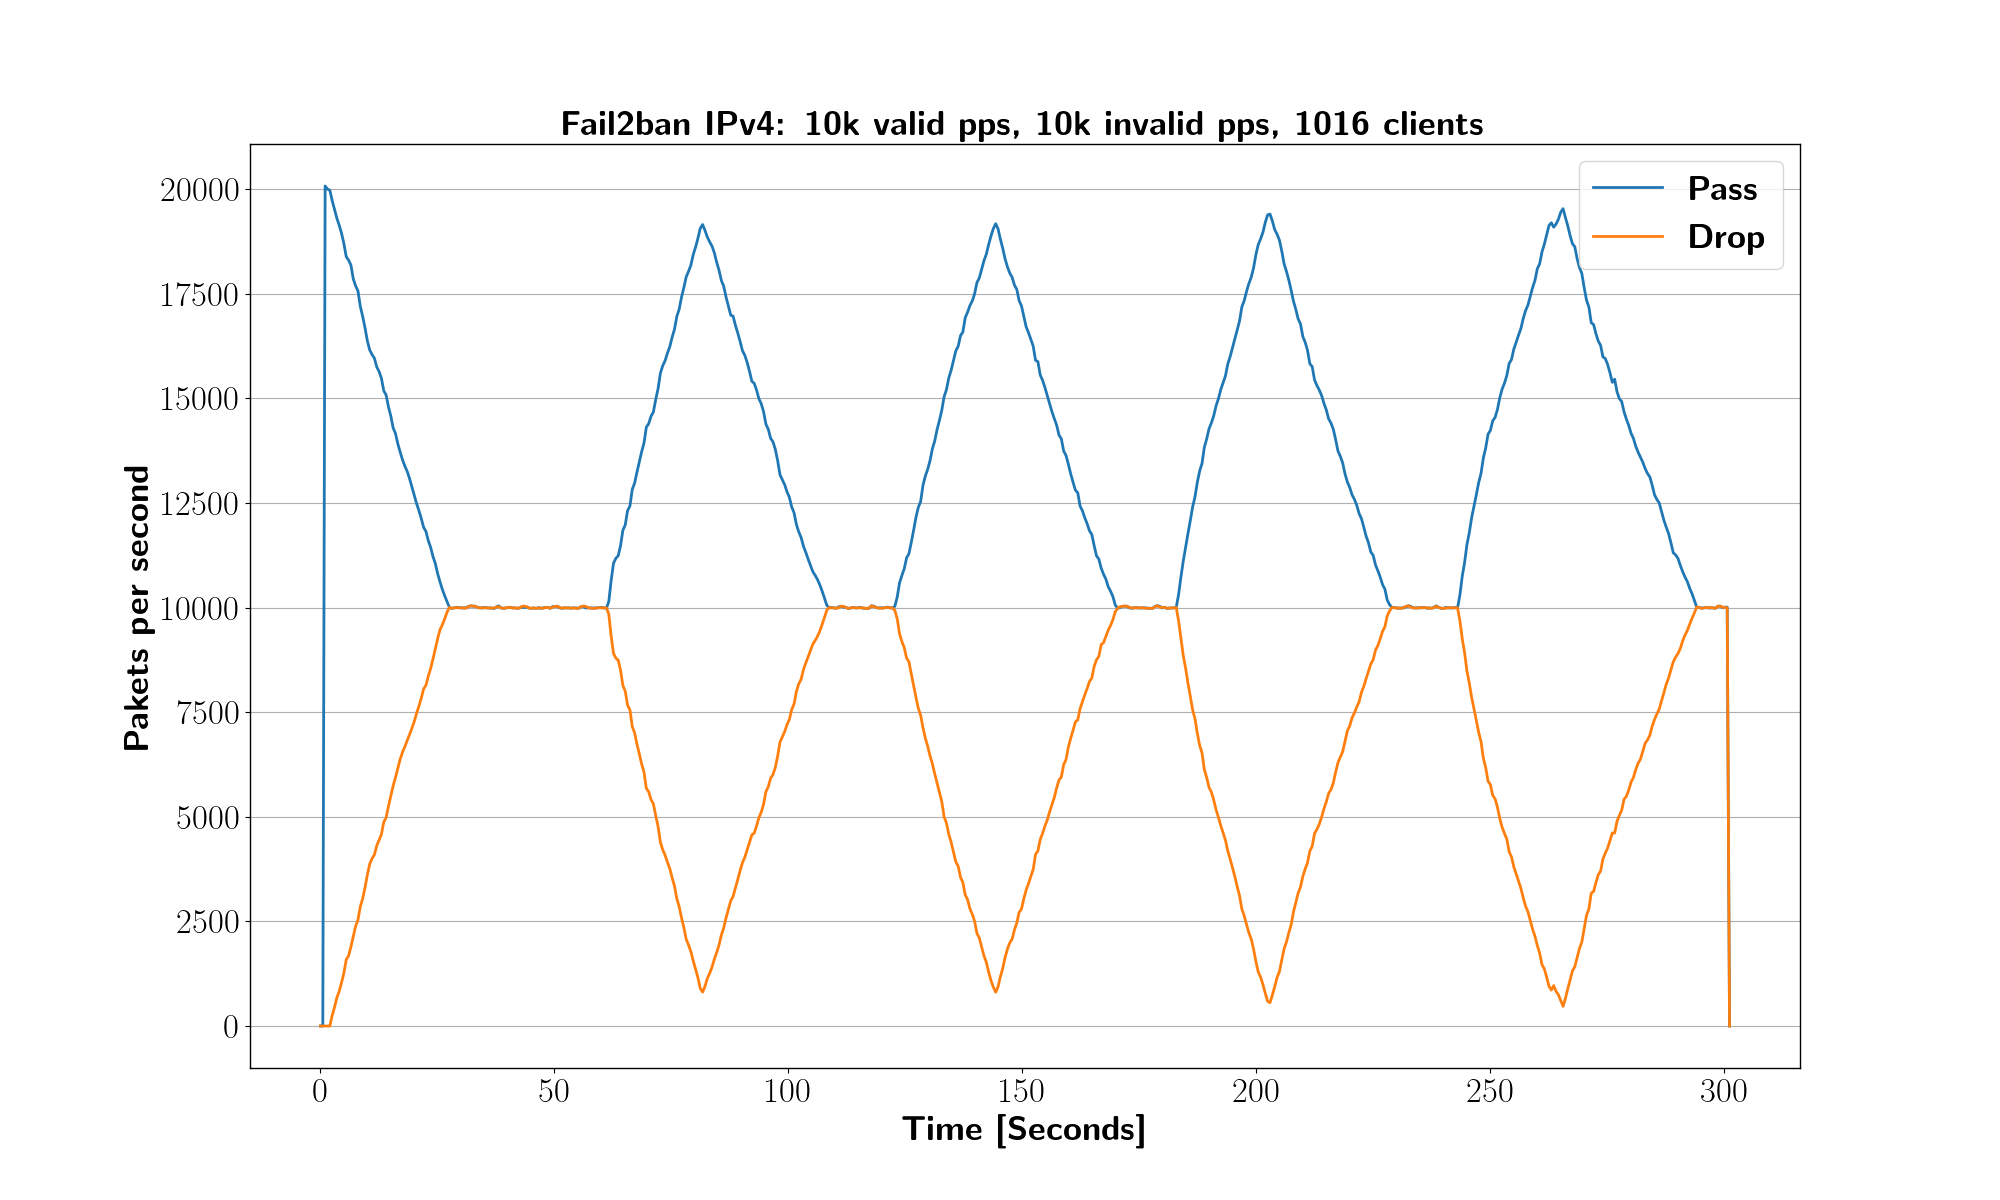
\includegraphics[width=1.2\textwidth]{images/fail2ban_v10k_iv10k_c1016.png}}
    \caption[Fail2Ban Replication Measurements 1]{Abstract architecture }
\end{figure}

\begin{figure}[p]
	\label{fig:fail2ban:1m}
    \centerline{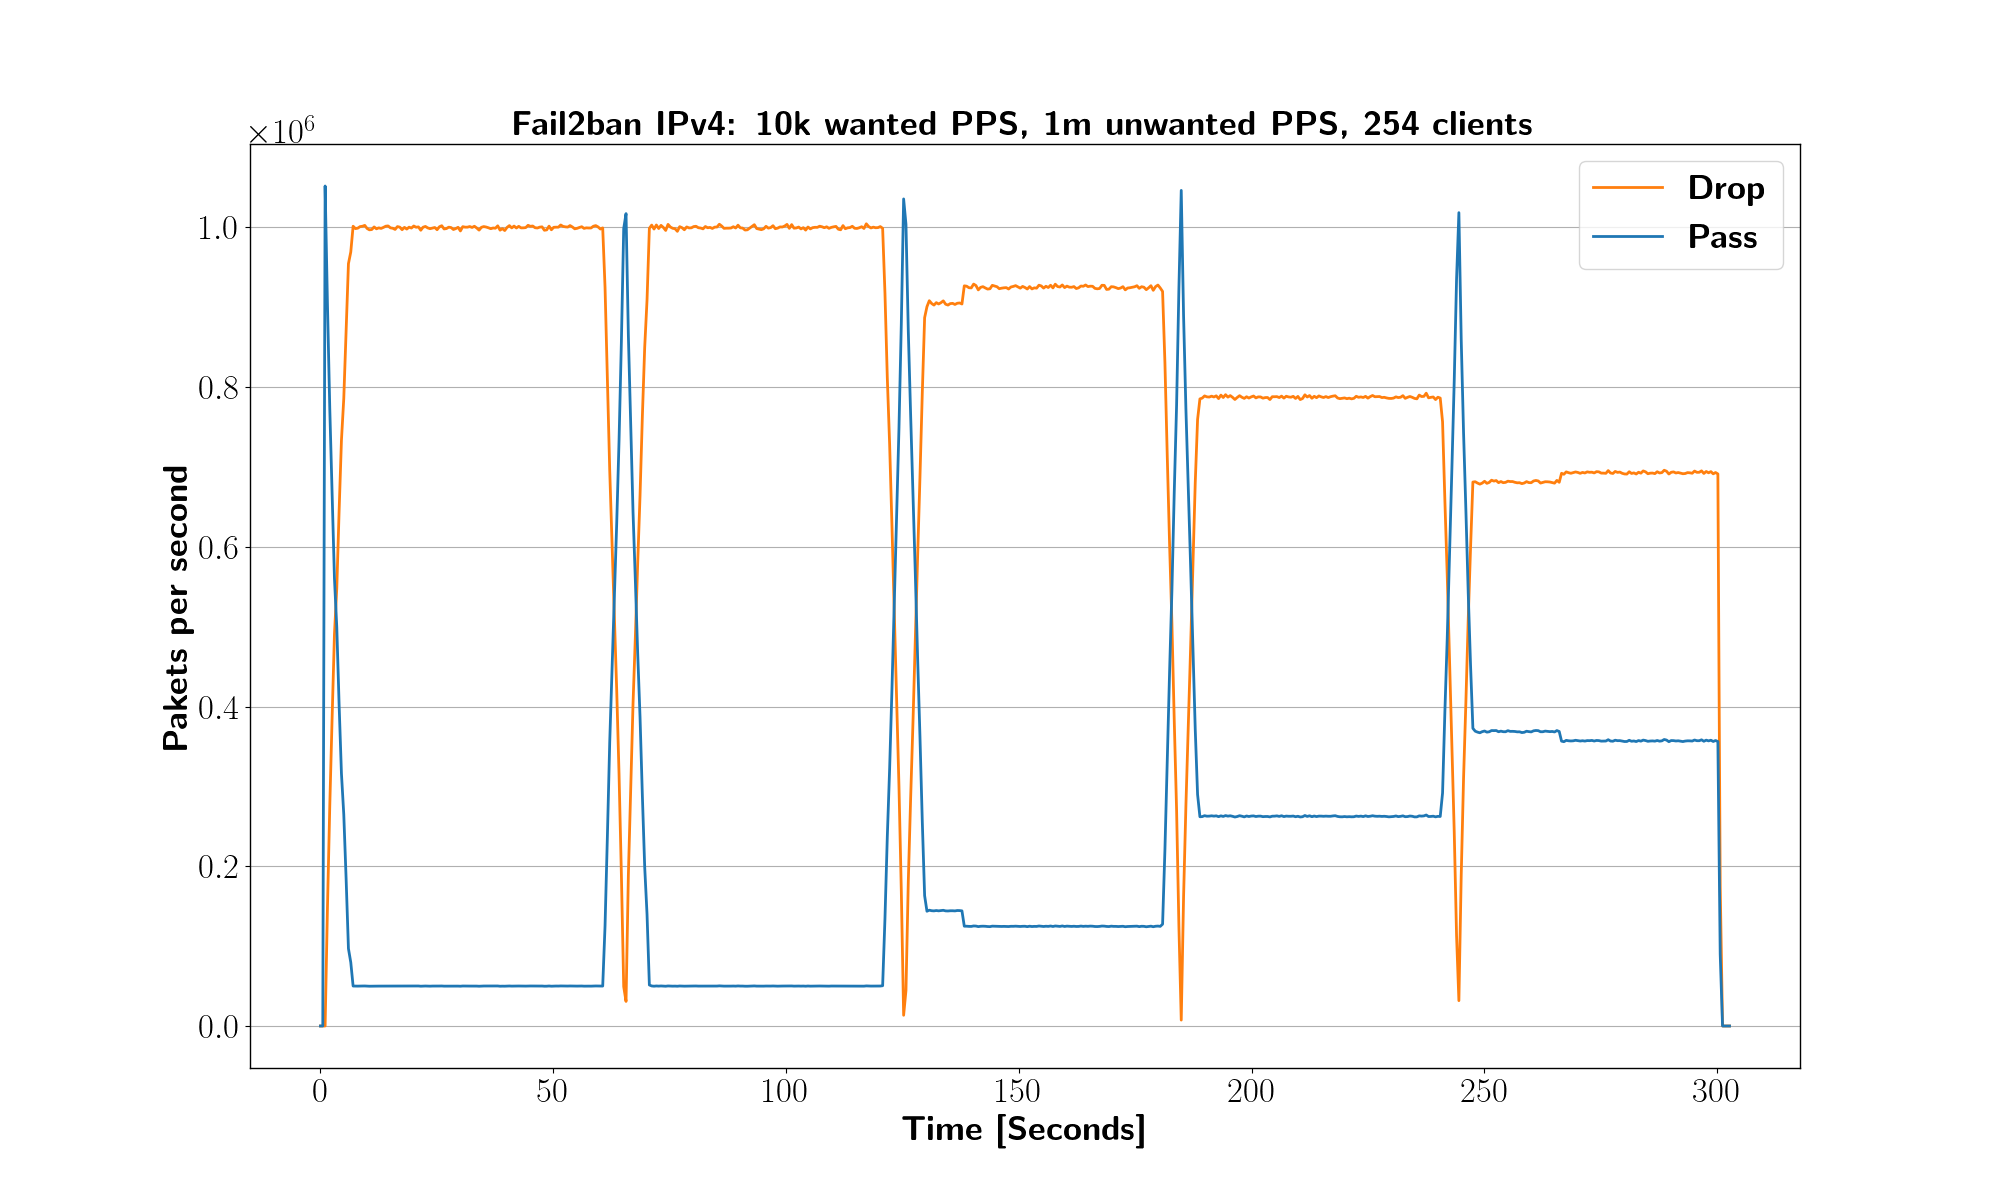
\includegraphics[width=1.2\textwidth]{images/fail2ban_v50k_iv1m_c254.png}}
    \caption[IPC Architecture]{Abstract architecture }
\end{figure}

\section{Simplefail2ban, Logfile Measurements}

\begin{figure}[p]
	\label{fig:simplefail2ban:disk:ip4:100k}
	\centering
	\scriptsize
	\begin{tabular}{c}
    	\centerline{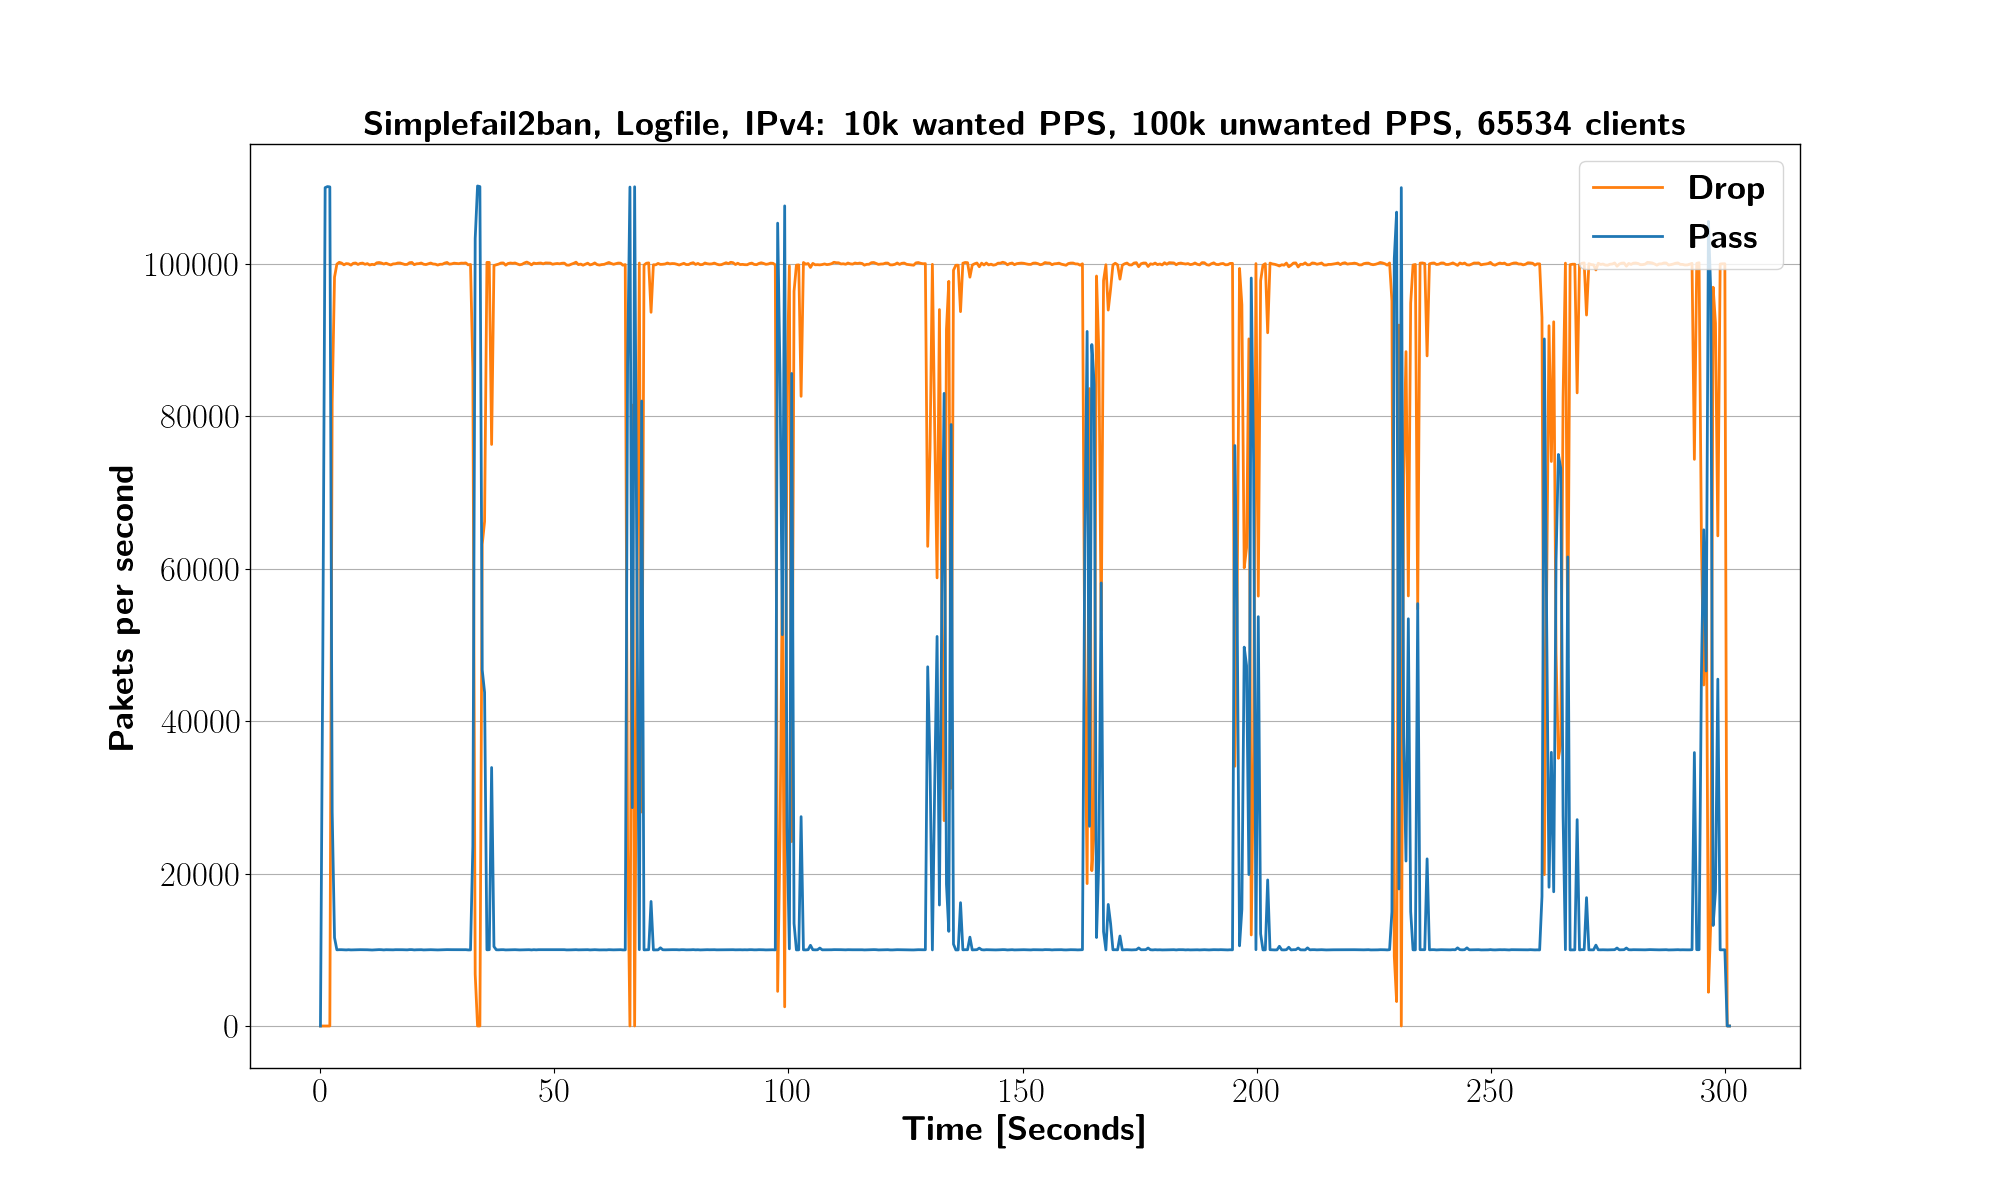
\includegraphics[width=1.2\textwidth]{images/simplefail2ban_disk_ipv4_v10k_iv100k_c65534.png}}
	\end{tabular}
	\begin{tabular}{lllll}
		\toprule
		\textbf{Total packets [$10^6$]} & \textbf{Packets dropped [$10^6$]} & \textbf{Relative drop [\%]} & \textbf{Log messages [$10^6$]} & \textbf{CPU [seconds]} \\ \midrule 
		33 & 27.93 & 99.59 & 2.07 & 10.51 \\
		\bottomrule
	\end{tabular}
	\caption[Simplefail2ban, Logfile IPv4, 100k \ac{PPS}]{Some text}
\end{figure}

\begin{figure}[p]
	\label{fig:simplefail2ban:disk:ip4:1m}
	\centering
	\scriptsize
	\begin{tabular}{c}
    	\centerline{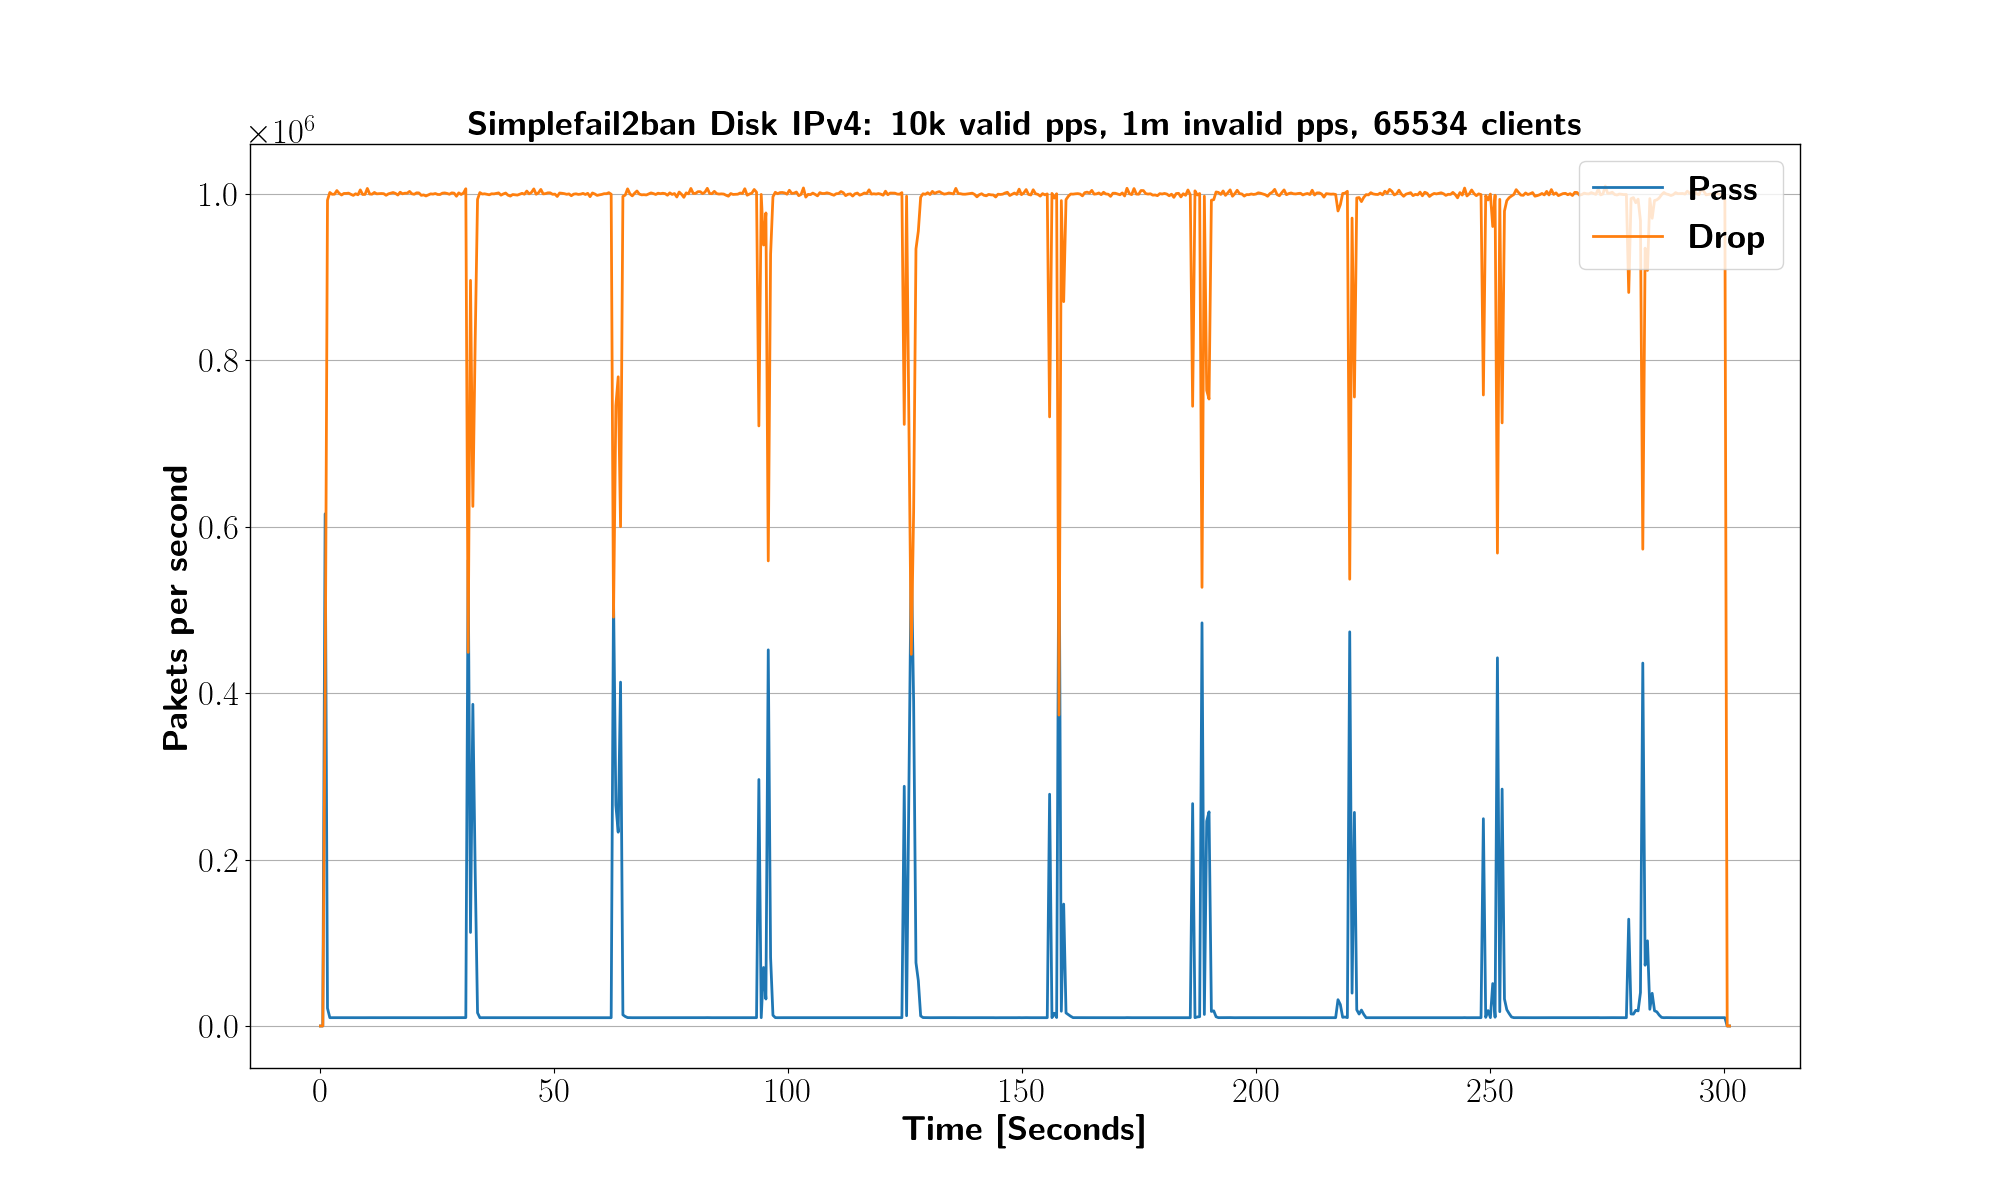
\includegraphics[width=1.2\textwidth]{images/simplefail2ban_disk_ipv4_v10k_iv1m_c65534.png}}
    \end{tabular}
	\begin{tabular}{lllll}
		\toprule
		\textbf{Total packets [$10^6$]} & \textbf{Packets dropped [$10^6$]} & \textbf{Relative drop [\%]} & \textbf{Log messages [$10^6$]} & \textbf{CPU [seconds]} \\ \midrule 
		303 & 294.43 & 98.79 & 4.7 & 14.99 \\
		\bottomrule
	\end{tabular}
	\caption[Simplefail2ban, Logfile IPv4, 1m \ac{PPS}]{Some text}
\end{figure}

\begin{figure}[p]
	\label{fig:simplefail2ban:disk:ip4:10m}
	\centering
	\scriptsize
	\begin{tabular}{c}
    	\centerline{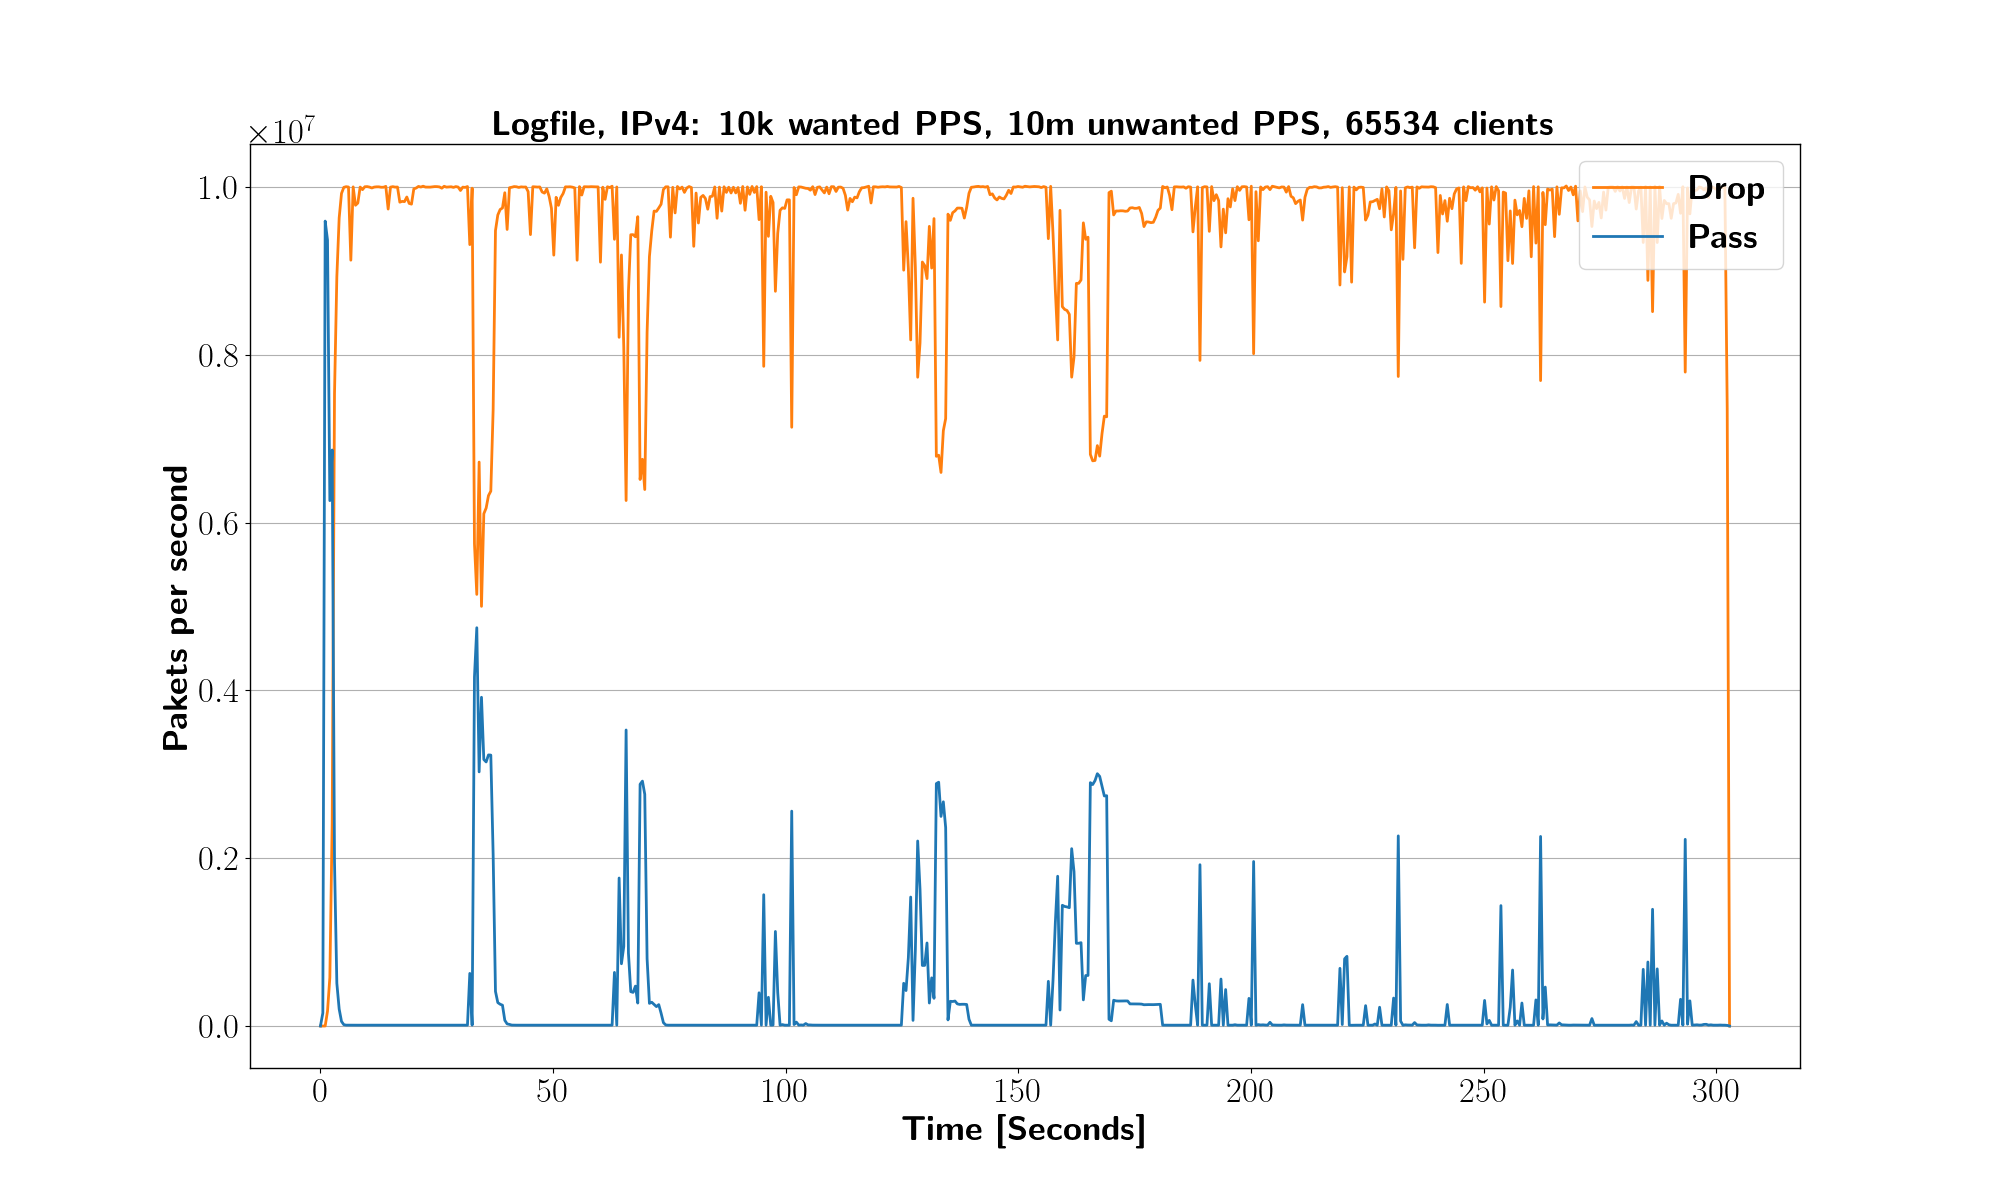
\includegraphics[width=1.2\textwidth]{images/simplefail2ban_disk_ipv4_v10k_iv10m_c65534.png}}
	\end{tabular}
	\begin{tabular}{lllll}
		\toprule
		\textbf{Total packets [$10^6$]} & \textbf{Packets dropped [$10^6$]} & \textbf{Relative drop [\%]} & \textbf{Log messages [$10^6$]} & \textbf{CPU [seconds]} \\ \midrule 
		2986.89 & 2884.14 & 96.72 & 34.39 & 83.72 \\
		\bottomrule
	\end{tabular}
	\caption[Simplefail2ban, Logfile IPv4, 10m \ac{PPS}]{Some text}
\end{figure}

\begin{figure}[p]
	\label{fig:simplefail2ban:disk:ip6:100k}
	\centering
	\scriptsize
	\begin{tabular}{c}
    	\centerline{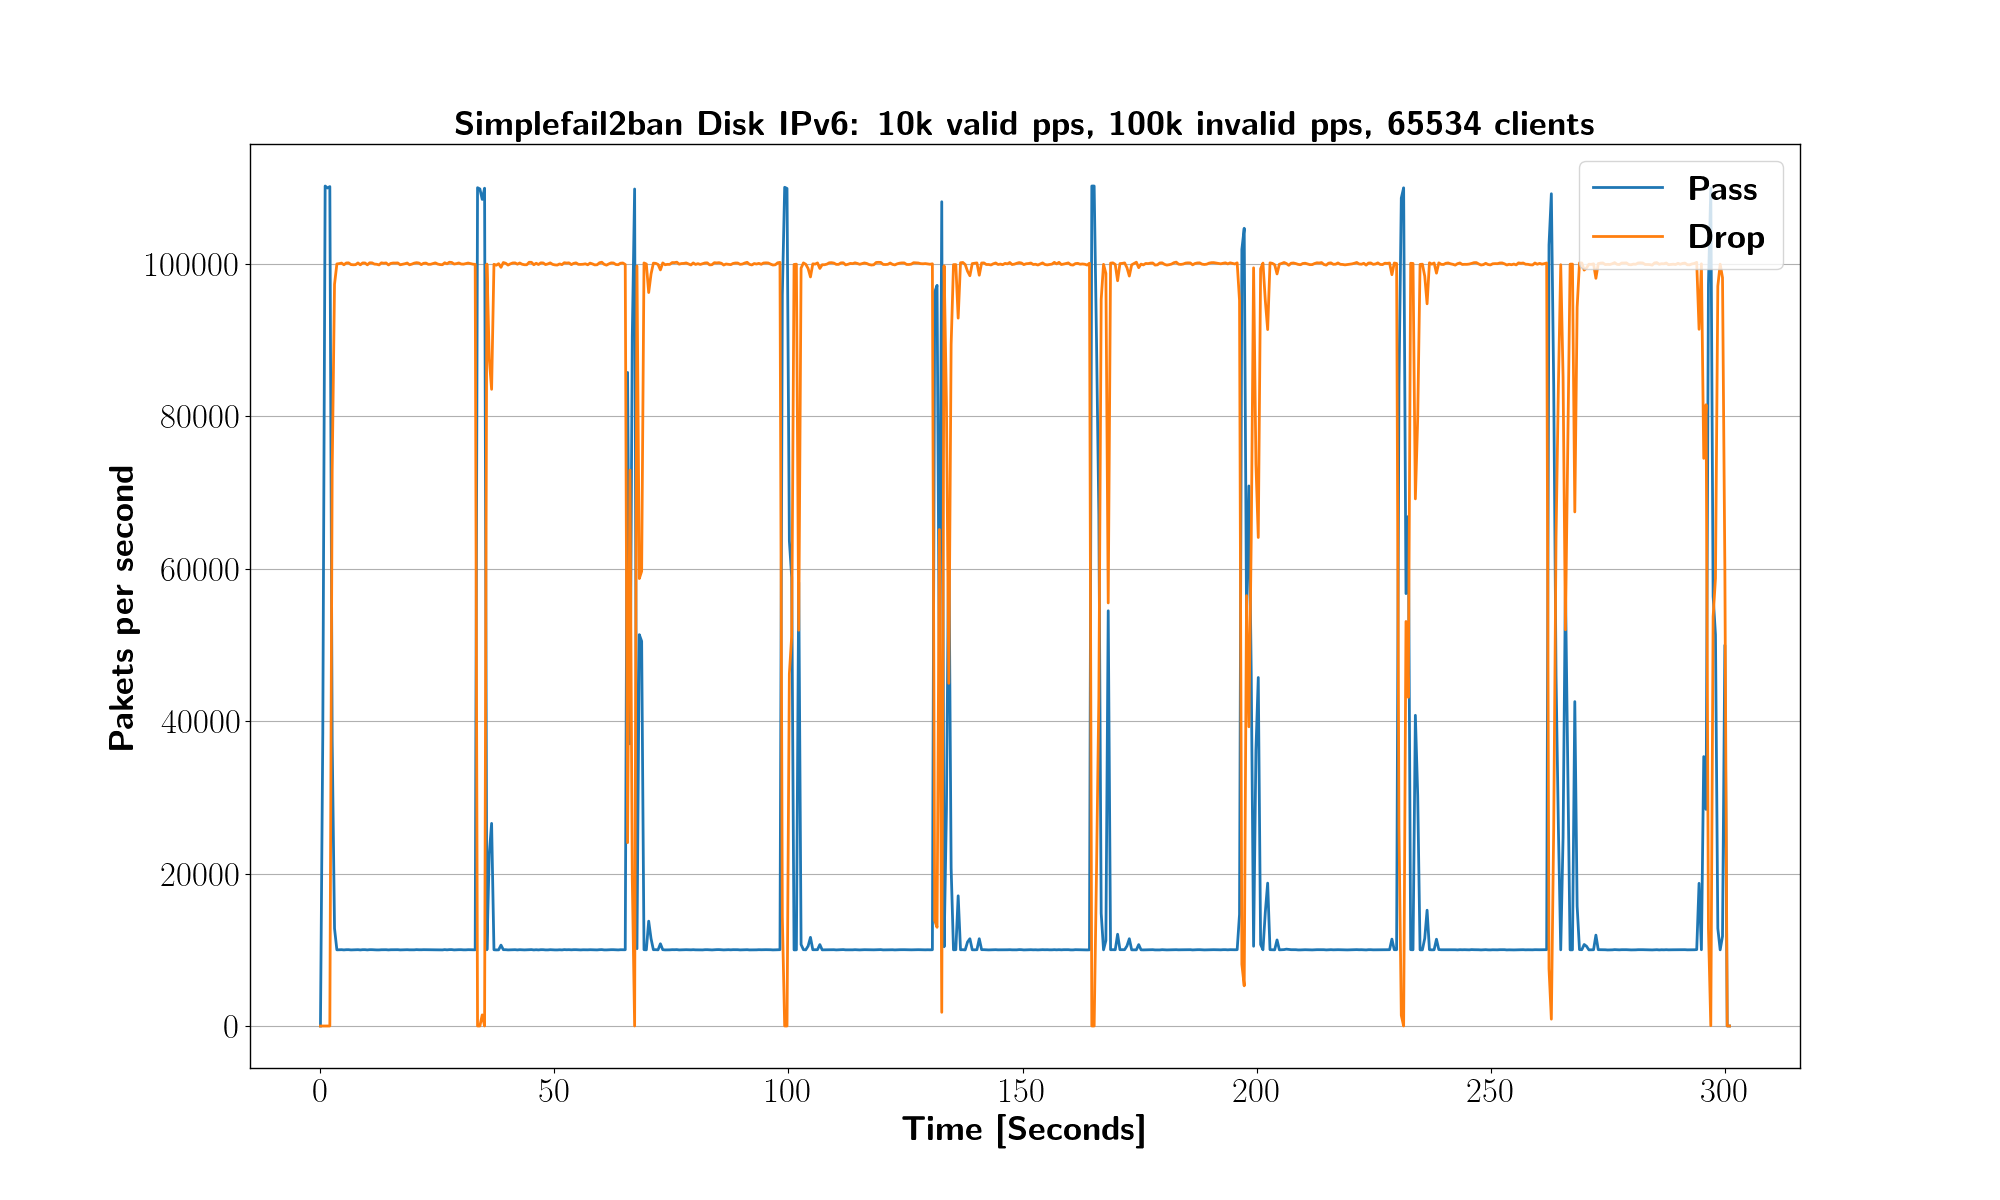
\includegraphics[width=1.2\textwidth]{images/simplefail2ban_disk_ipv6_v10k_iv100k_c65534.png}}
	\end{tabular}
	\begin{tabular}{lllll}
		\toprule
		\textbf{Total packets [$10^6$]} & \textbf{Packets dropped [$10^6$]} & \textbf{Relative drop [\%]} & \textbf{Log messages [$10^6$]} & \textbf{CPU [seconds]} \\ \midrule 
		33 & 27.96 & 99.67 & 2.04 & 11.75 \\
		\bottomrule
	\end{tabular}
	\caption[Simplefail2ban, Logfile IPv6, 100k \ac{PPS}]{Some text}
\end{figure}

\begin{figure}[p]
	\label{fig:simplefail2ban:disk:ip6:1m}
	\centering
	\scriptsize
	\begin{tabular}{c}
    	\centerline{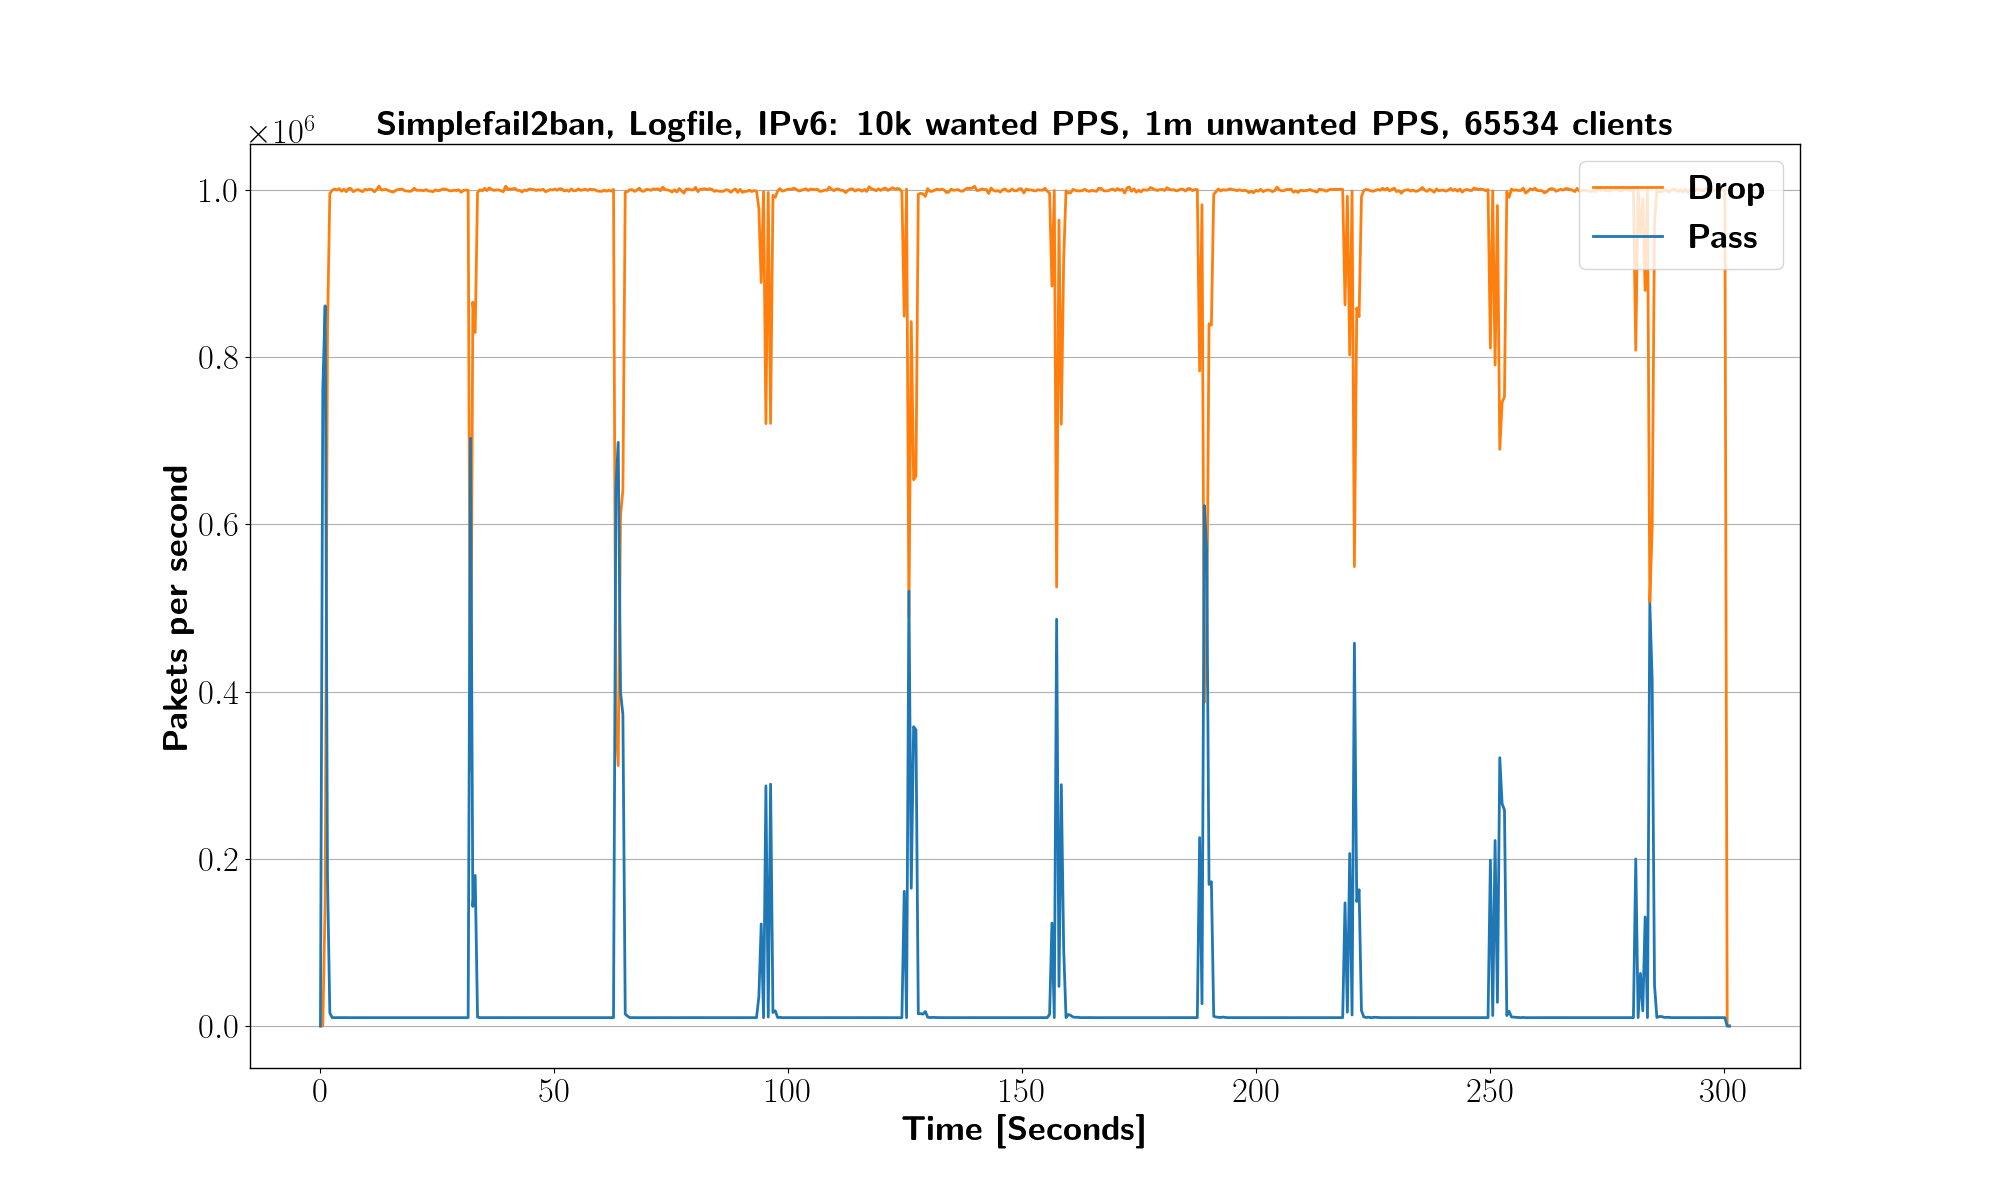
\includegraphics[width=1.2\textwidth]{images/simplefail2ban_disk_ipv6_v10k_iv1m_c65534.png}}
	\end{tabular}
	\begin{tabular}{lllll}
		\toprule
		\textbf{Total packets [$10^6$]} & \textbf{Packets dropped [$10^6$]} & \textbf{Relative drop [\%]} & \textbf{Log messages [$10^6$]} & \textbf{CPU [seconds]} \\ \midrule 
		303 & 293.49 & 98.48 & 5.58 & 21.08 \\
		\bottomrule
	\end{tabular}
	\caption[Simplefail2ban, Logfile IPv6, 1m \ac{PPS}]{Some text}
\end{figure}

\begin{figure}[p]
	\label{fig:simplefail2ban:disk:ip6:10m}
	\centering
	\scriptsize
	\begin{tabular}{c}
    	\centerline{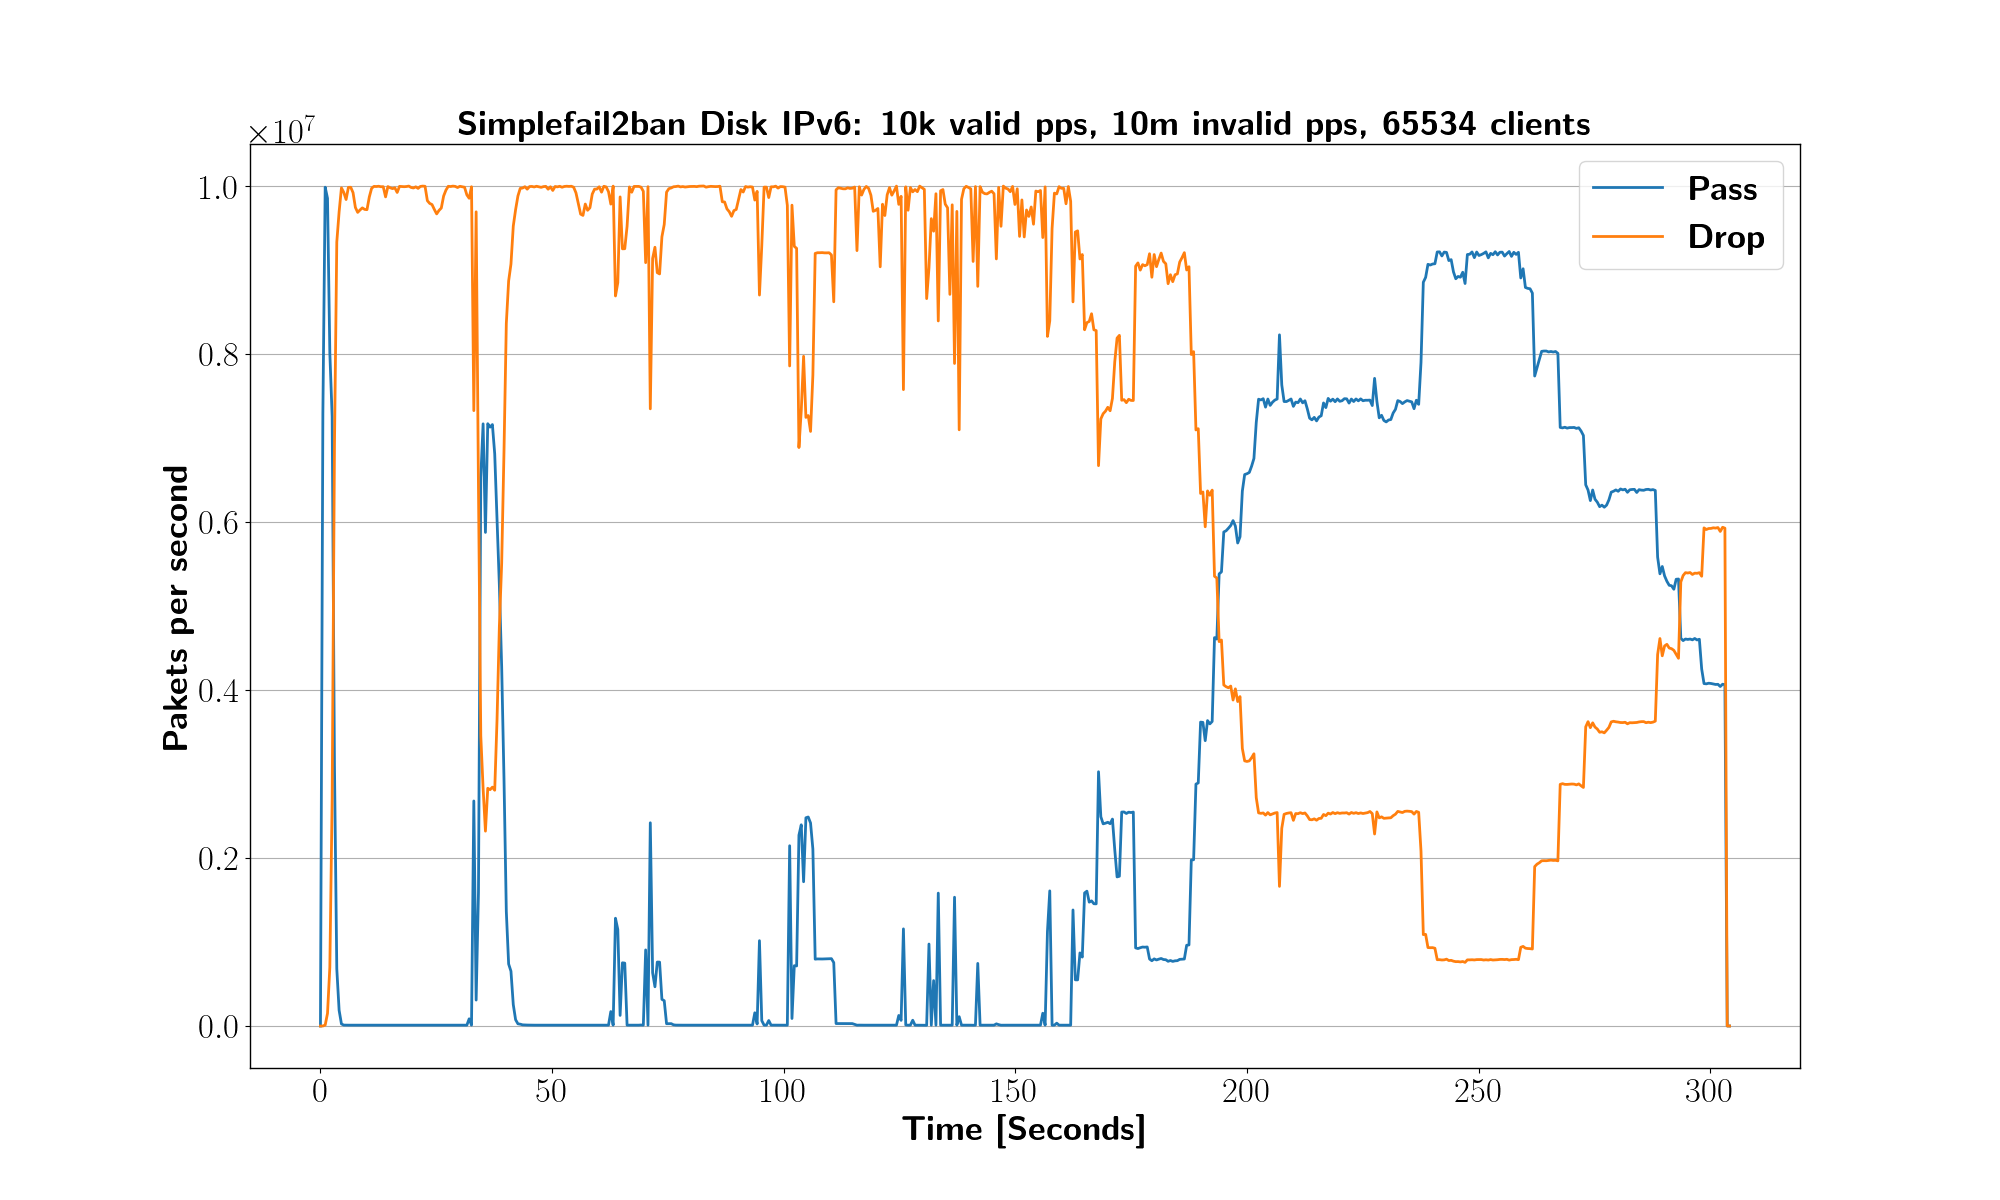
\includegraphics[width=1.2\textwidth]{images/simplefail2ban_disk_ipv6_v10k_iv10m_c65534.png}}
	\end{tabular}
	\begin{tabular}{lllll}
		\toprule
		\textbf{Total packets [$10^6$]} & \textbf{Packets dropped [$10^6$]} & \textbf{Relative drop [\%]} & \textbf{Log messages [$10^6$]} & \textbf{CPU [seconds]} \\ \midrule 
		2992.43 & 2065.28 & 69.13 & 205.4 & 346.73 \\
		\bottomrule
	\end{tabular}
	\caption[Simplefail2ban, Logfile IPv6, 10m \ac{PPS}]{Some text}
\end{figure}

\begin{figure}[p]
	\label{fig:simplefail2ban:disk:ip46:100k}
	\centering
	\scriptsize
	\begin{tabular}{c}
    	\centerline{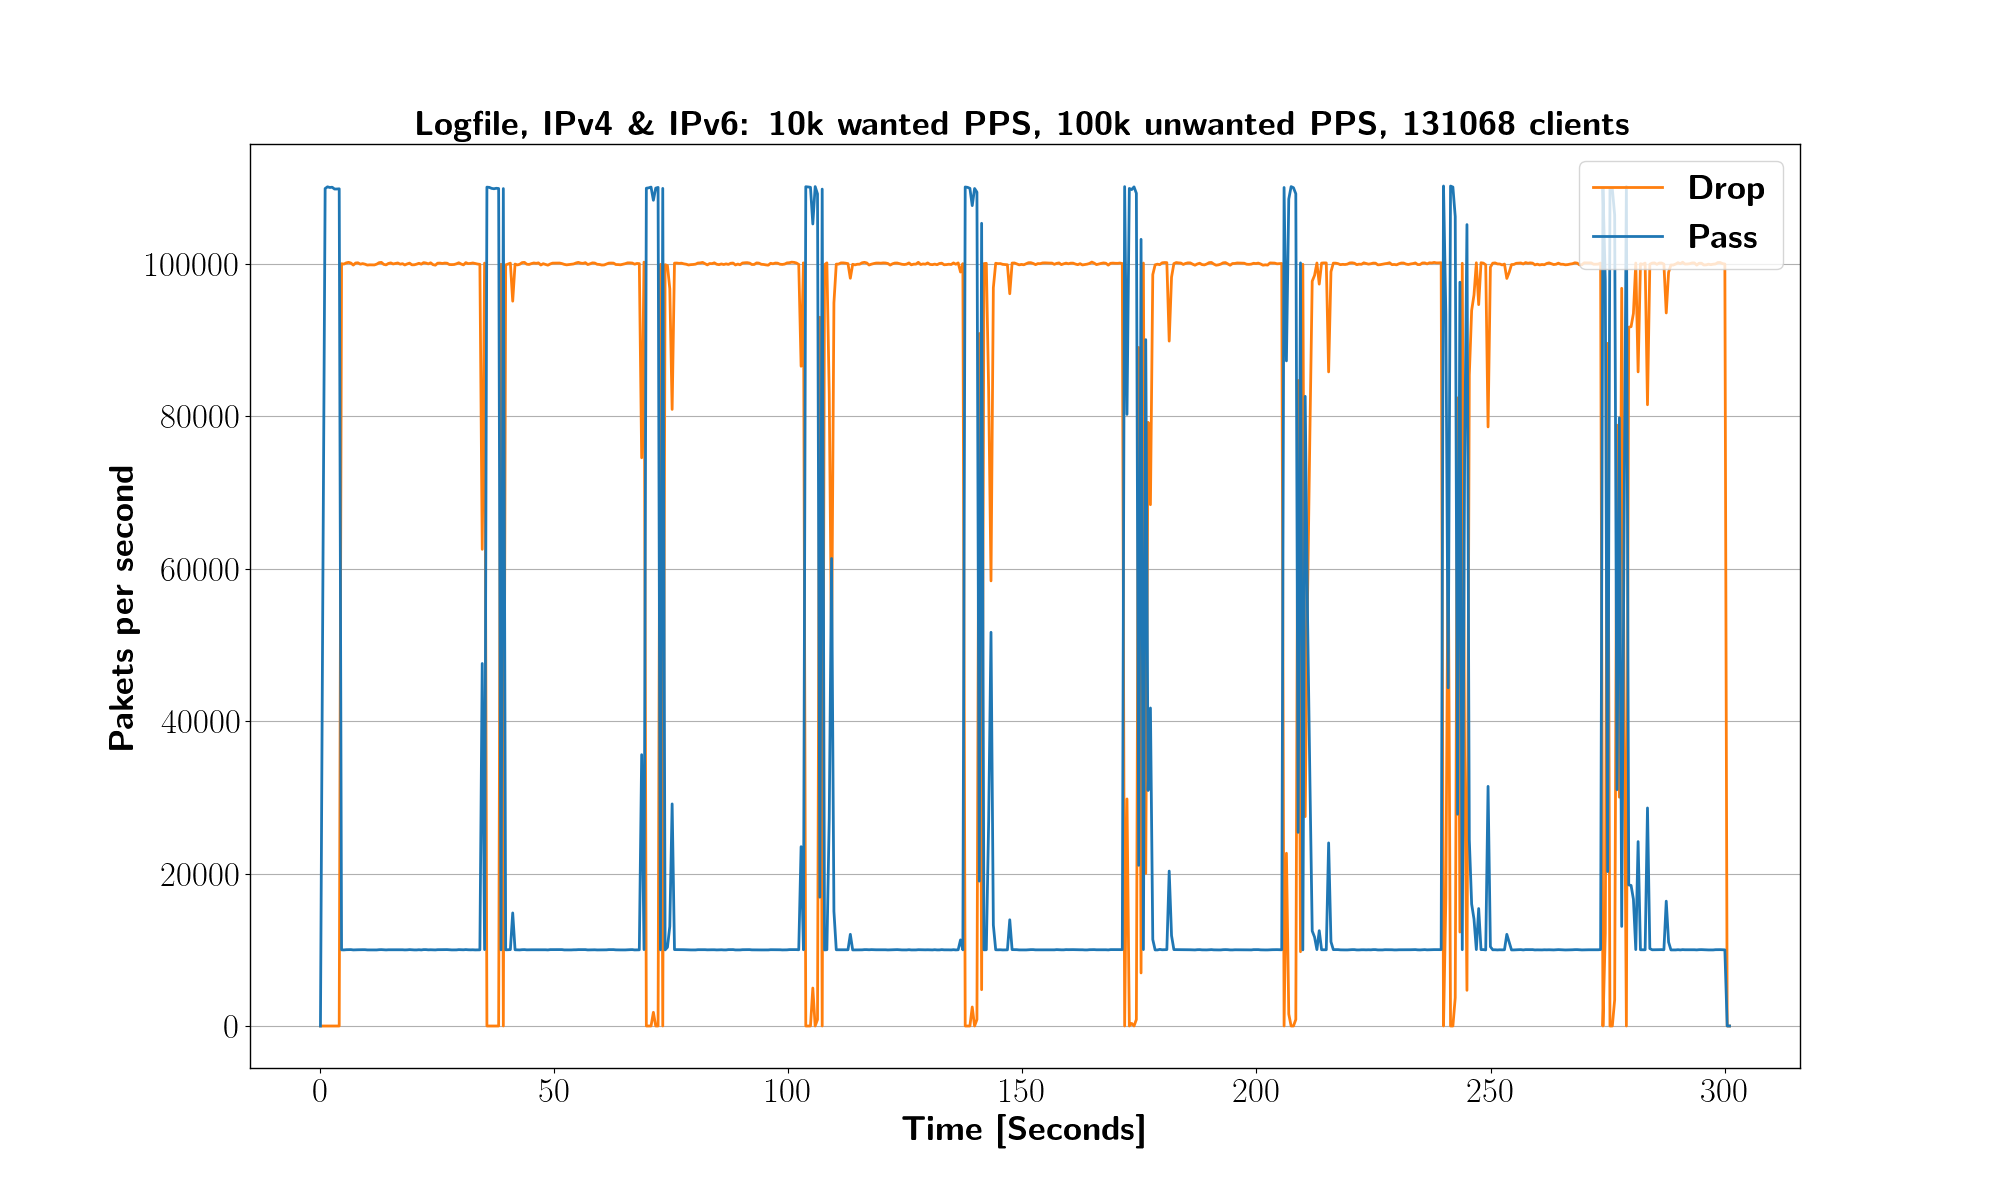
\includegraphics[width=1.2\textwidth]{images/simplefail2ban_disk_ipv46_v10k_iv100k_c131068.png}}
	\end{tabular}
	\begin{tabular}{lllll}
		\toprule
		\textbf{Total packets [$10^6$]} & \textbf{Packets dropped [$10^6$]} & \textbf{Relative drop [\%]} & \textbf{Log messages [$10^6$]} & \textbf{CPU [seconds]} \\ \midrule 
		33 & 26.45 & 99.96 & 3.55 & 18.47 \\
	\bottomrule
	\end{tabular}
	\caption[Simplefail2ban, Logfile IPv4 \& IPv6, 100k \ac{PPS}]{Some text}
\end{figure}

\begin{figure}[p]
	\label{fig:simplefail2ban:disk:ip46:1m}
	\centering
	\scriptsize
	\begin{tabular}{c}
    	\centerline{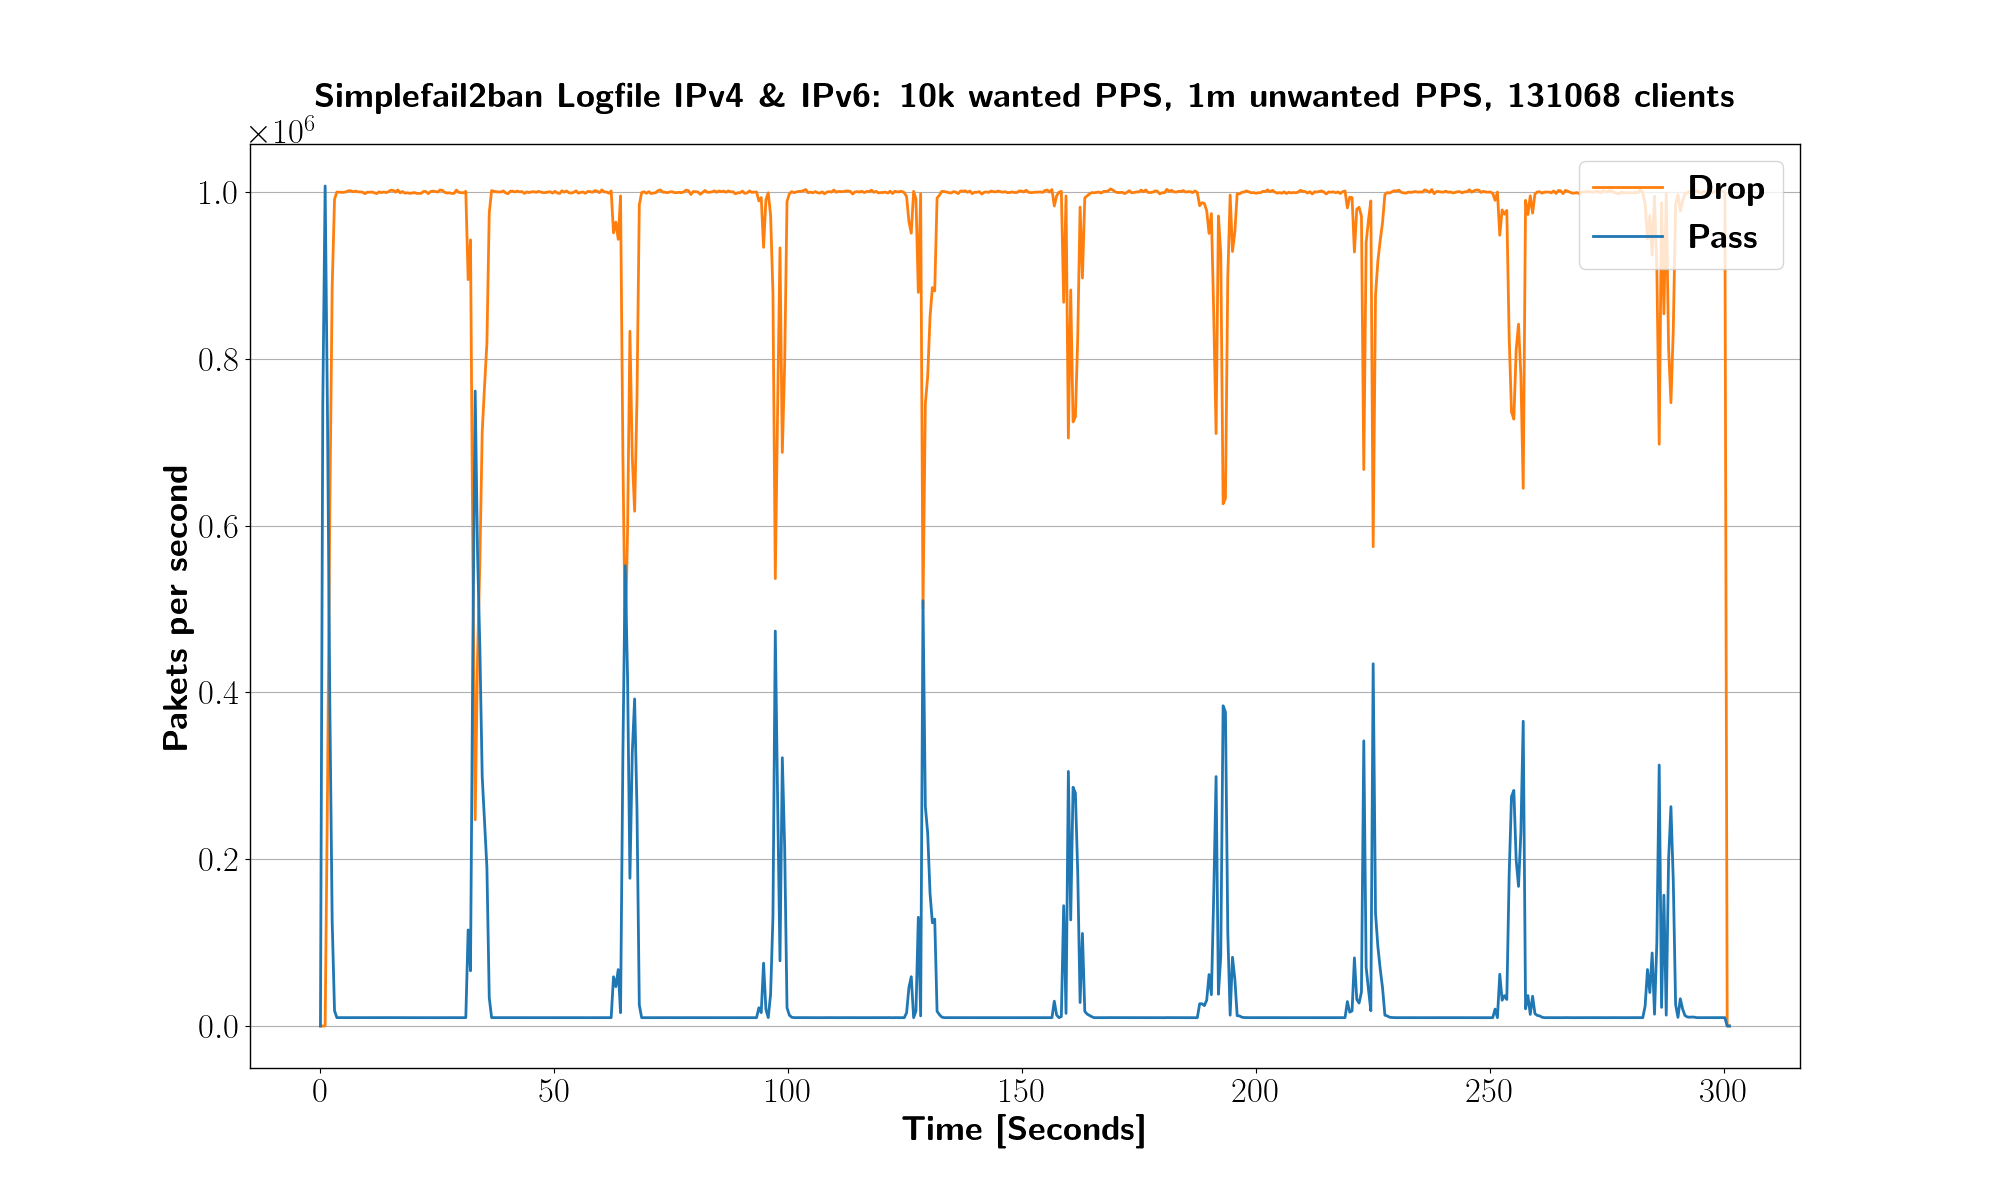
\includegraphics[width=1.2\textwidth]{images/simplefail2ban_disk_ipv46_v10k_iv1m_c131068.png}}
	\end{tabular}
	\begin{tabular}{lllll}
		\toprule
		\textbf{Total packets [$10^6$]} & \textbf{Packets dropped [$10^6$]} & \textbf{Relative drop [\%]} & \textbf{Log messages [$10^6$]} & \textbf{CPU [seconds]} \\ \midrule 
		303 & 290.47 & 98.11 & 8.5 & 32.94 \\
	\bottomrule
	\end{tabular}
	\caption[Simplefail2ban, Logfile IPv4 \& IPv6, 1m \ac{PPS}]{Some text}
\end{figure}

\begin{figure}[p]
	\label{fig:simplefail2ban:disk:ip46:10m}
	\centering
	\scriptsize
	\begin{tabular}{c}
    	\centerline{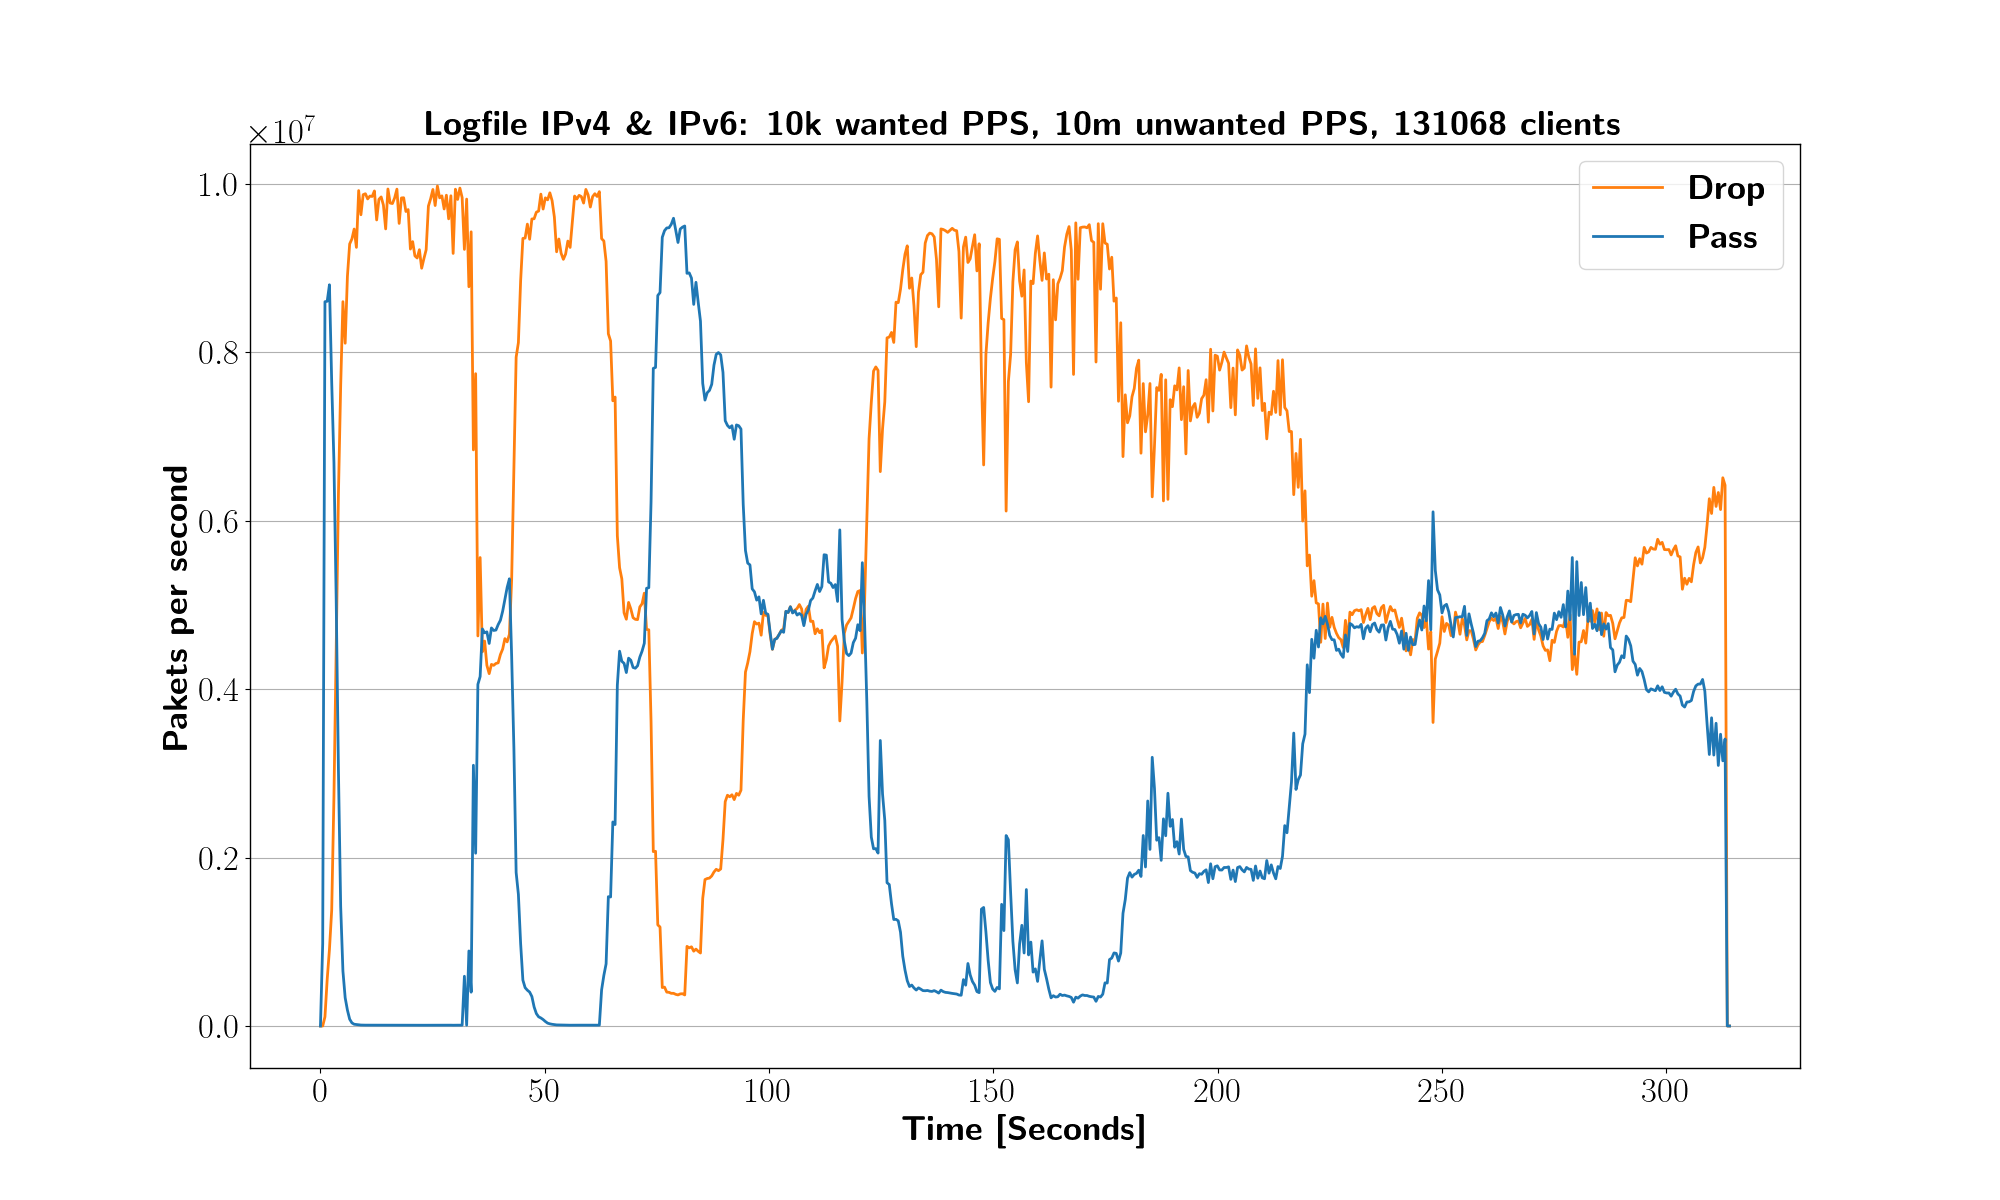
\includegraphics[width=1.2\textwidth]{images/simplefail2ban_disk_ipv46_v10k_iv10m_c131068.png}}
	\end{tabular}
	\begin{tabular}{lllll}
		\toprule
		\textbf{Total packets [$10^6$]} & \textbf{Packets dropped [$10^6$]} & \textbf{Relative drop [\%]} & \textbf{Log messages [$10^6$]} & \textbf{CPU [seconds]} \\ \midrule 
		2993.57 & 2014.77 & 67.46 & 213.63 & 382.19 \\
		\bottomrule
	\end{tabular}
	\caption[Simplefail2ban, Logfile IPv4 \& IPv6, 10m \ac{PPS}]{Some text}
\end{figure}

\section{Simplefail2ban, Shared Memory Measurements}

\begin{figure}[p]
	\label{fig:simplefail2ban:shm:ip4:100k}
	\centering
	\scriptsize
	\begin{tabular}{c}
    	\centerline{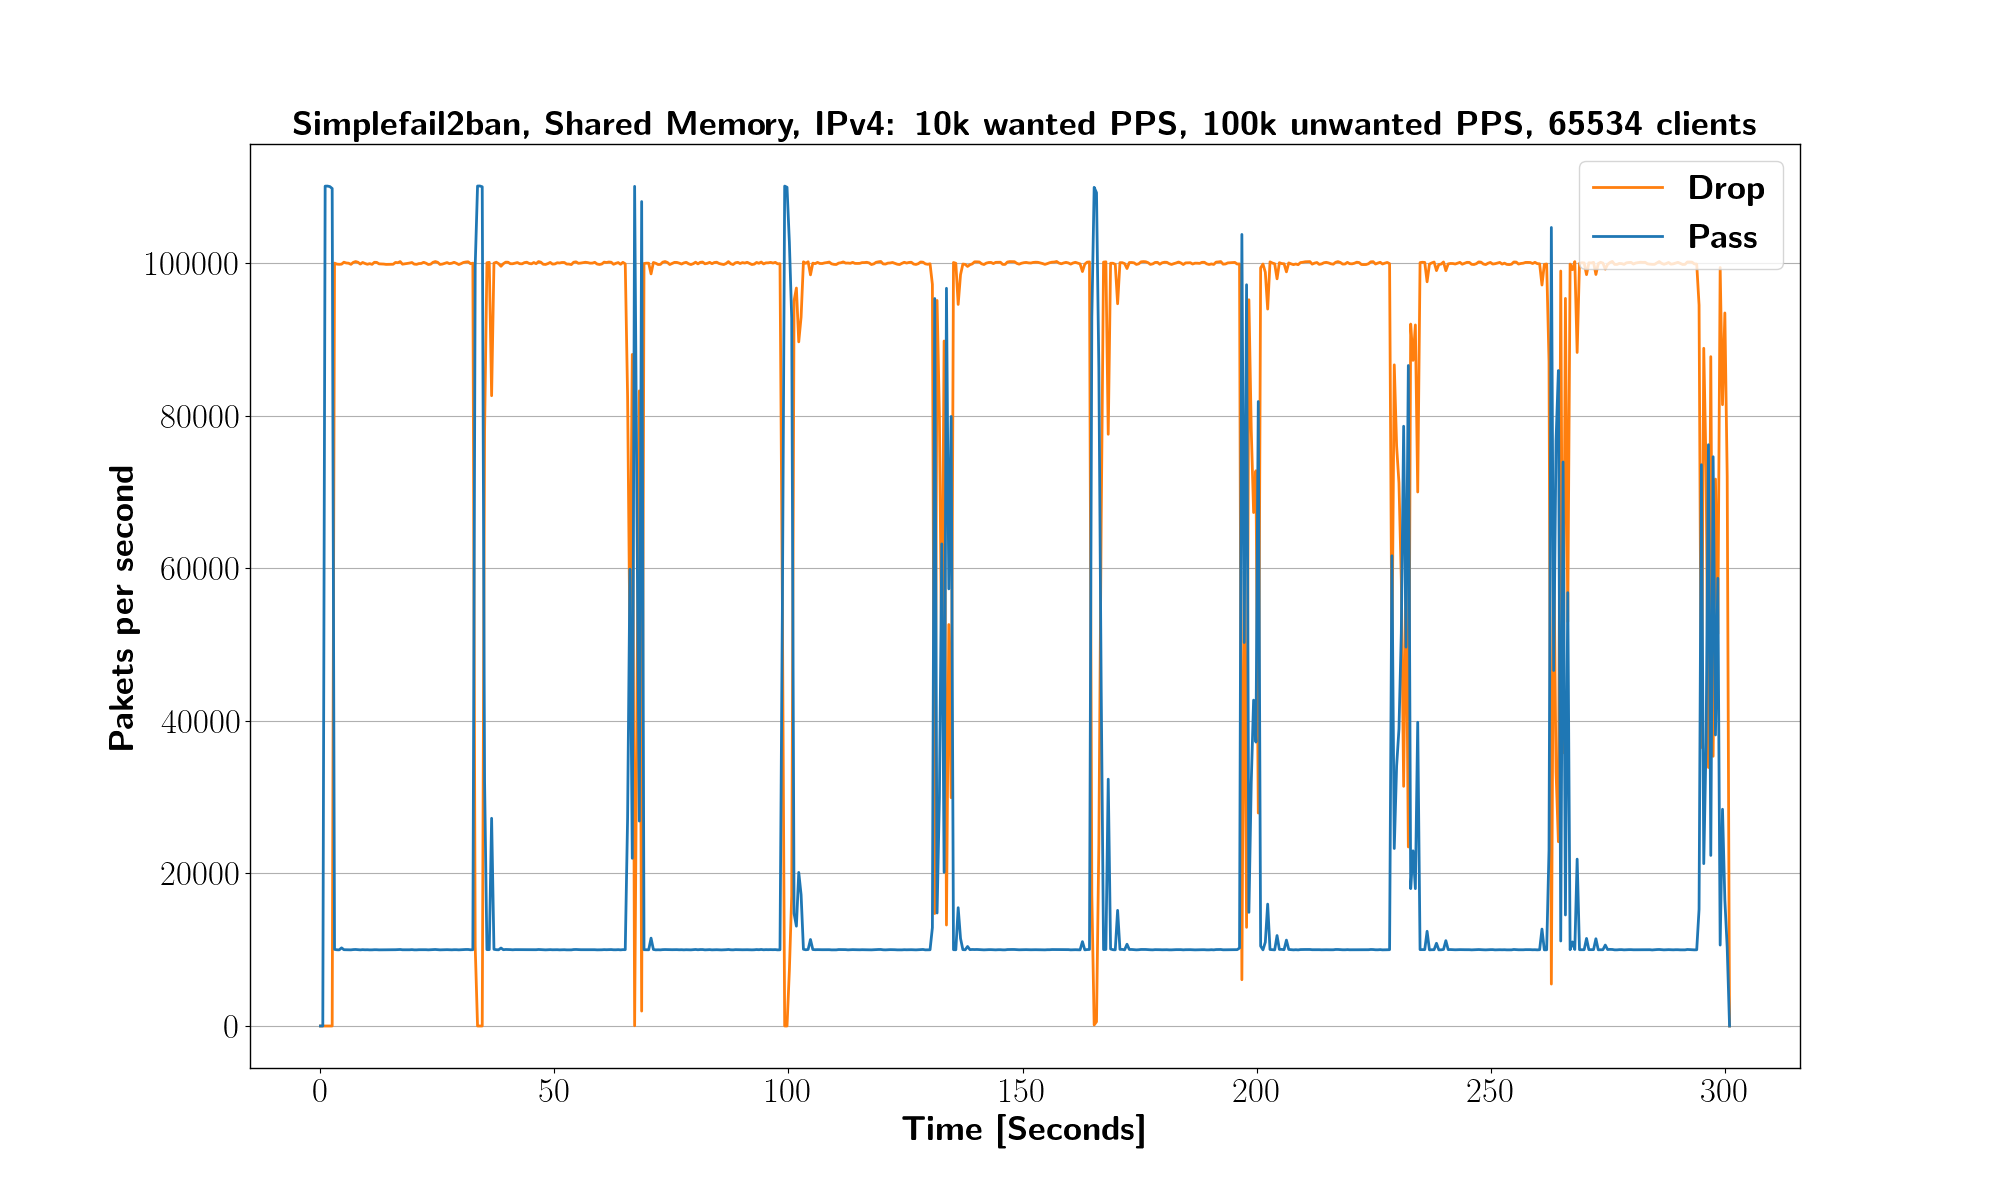
\includegraphics[width=1.2\textwidth]{images/simplefail2ban_shm_ipv4_v10k_iv100k_c65534.png}}
	\end{tabular}
	\begin{tabular}{lllll}
		\toprule
		\textbf{Total packets [$10^6$]} & \textbf{Packets dropped [$10^6$]} & \textbf{Relative drop [\%]} & \textbf{Log messages [$10^6$]} & \textbf{CPU [seconds]} \\ \midrule 
		33 & 27.95 & 99.64 & 2.05 & 13.68 \\
		\bottomrule
	\end{tabular}
	\caption[Simplefail2ban, Shared Memory, IPv4, 1m \ac{PPS}]{Some text}
\end{figure}

\begin{figure}[p]
	\label{fig:simplefail2ban:shm:ip4:1m}
	\centering
	\scriptsize
	\begin{tabular}{c}
    	\centerline{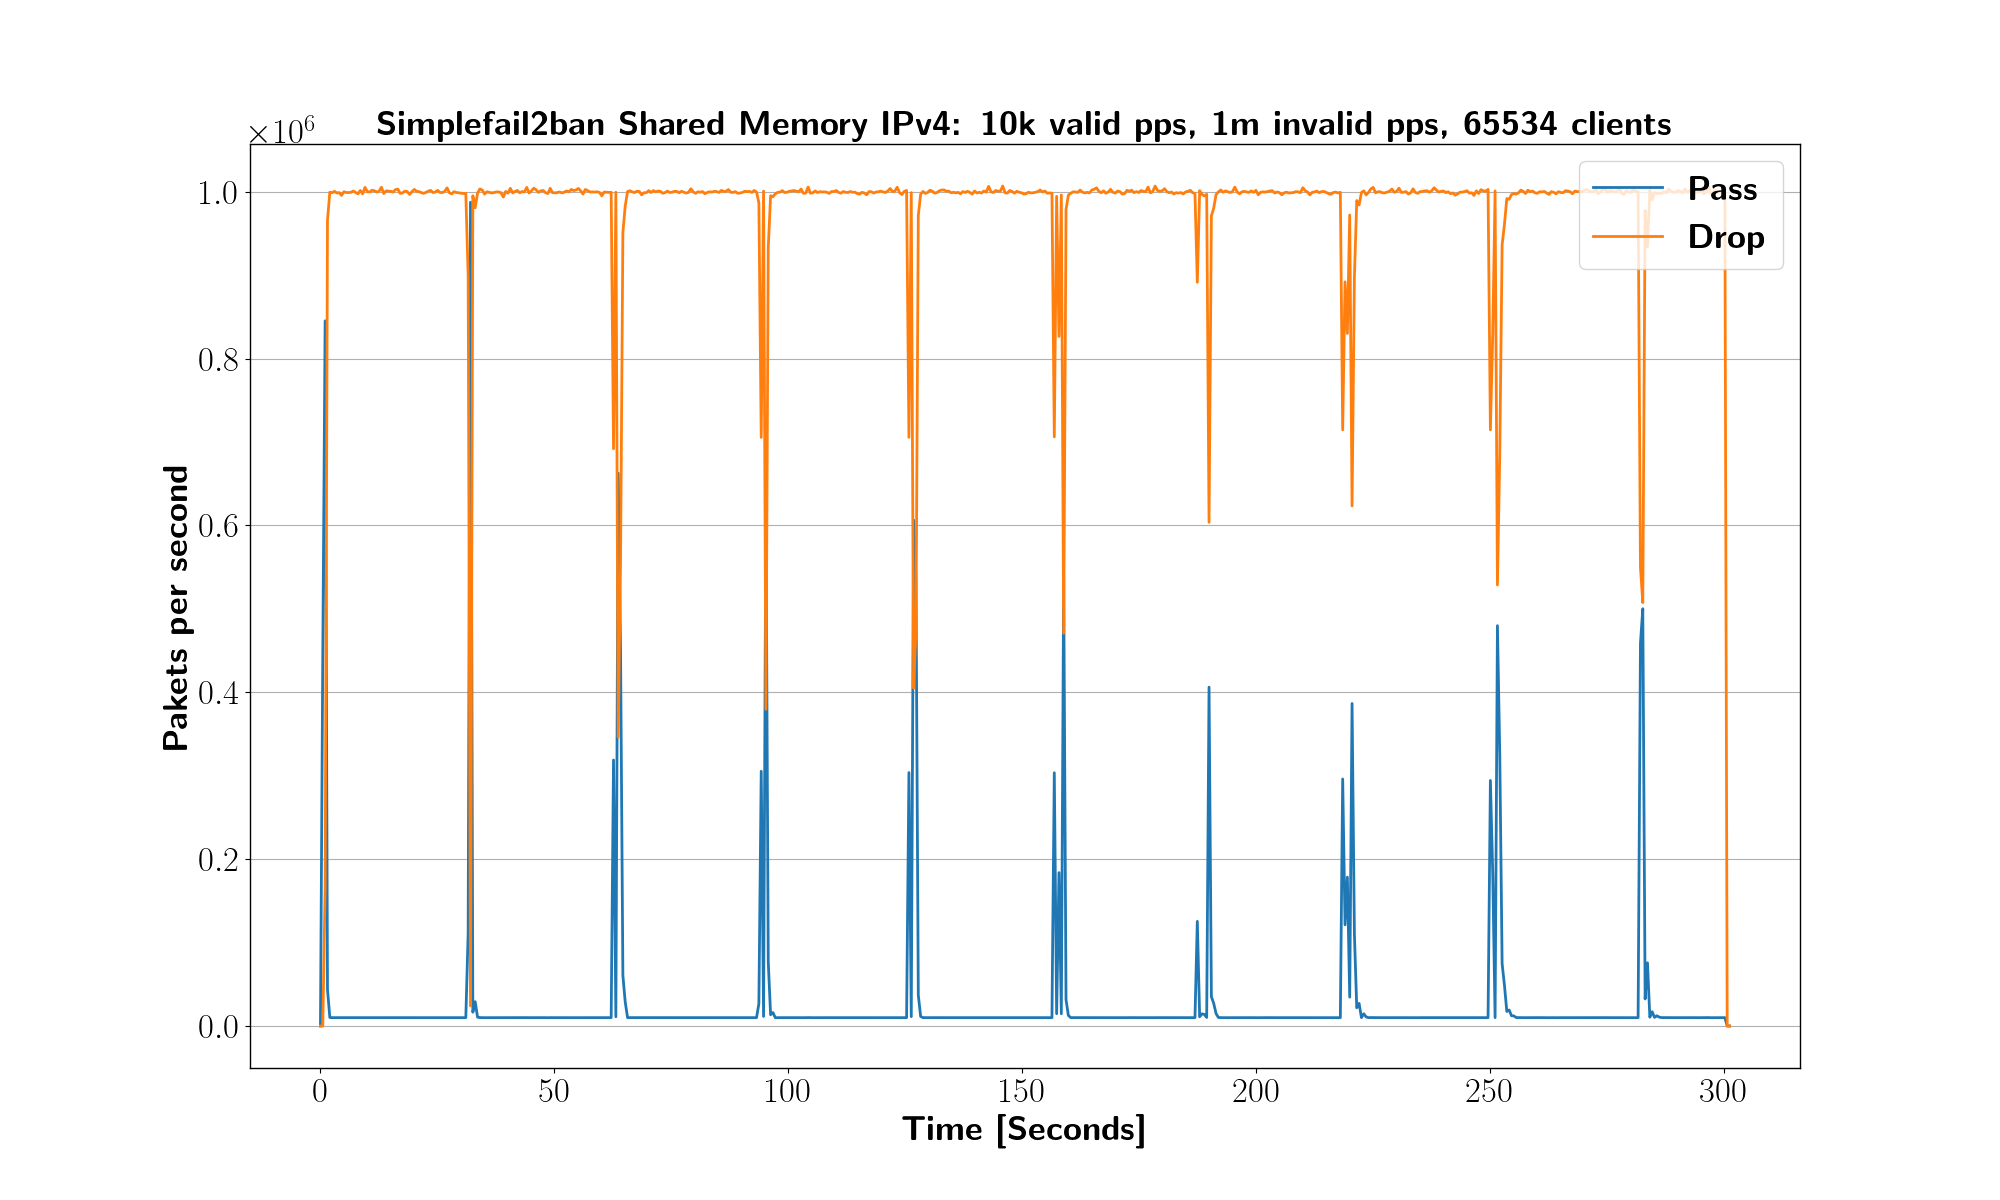
\includegraphics[width=1.2\textwidth]{images/simplefail2ban_shm_ipv4_v10k_iv1m_c65534.png}}
	\end{tabular}
	\begin{tabular}{lllll}
		\toprule
		\textbf{Total packets [$10^6$]} & \textbf{Packets dropped [$10^6$]} & \textbf{Relative drop [\%]} & \textbf{Log messages [$10^6$]} & \textbf{CPU [seconds]} \\ \midrule 
		303 & 294.34 & 98.88 & 4.61 & 15.52 \\
		\bottomrule
	\end{tabular}
	\caption[Simplefail2ban, Shared Memory, IPv4, 1m \ac{PPS}]{Some text}
\end{figure}

\begin{figure}[p]
	\label{fig:simplefail2ban:shm:ip4:10m}
	\centering
	\scriptsize
	\begin{tabular}{c}
    	\centerline{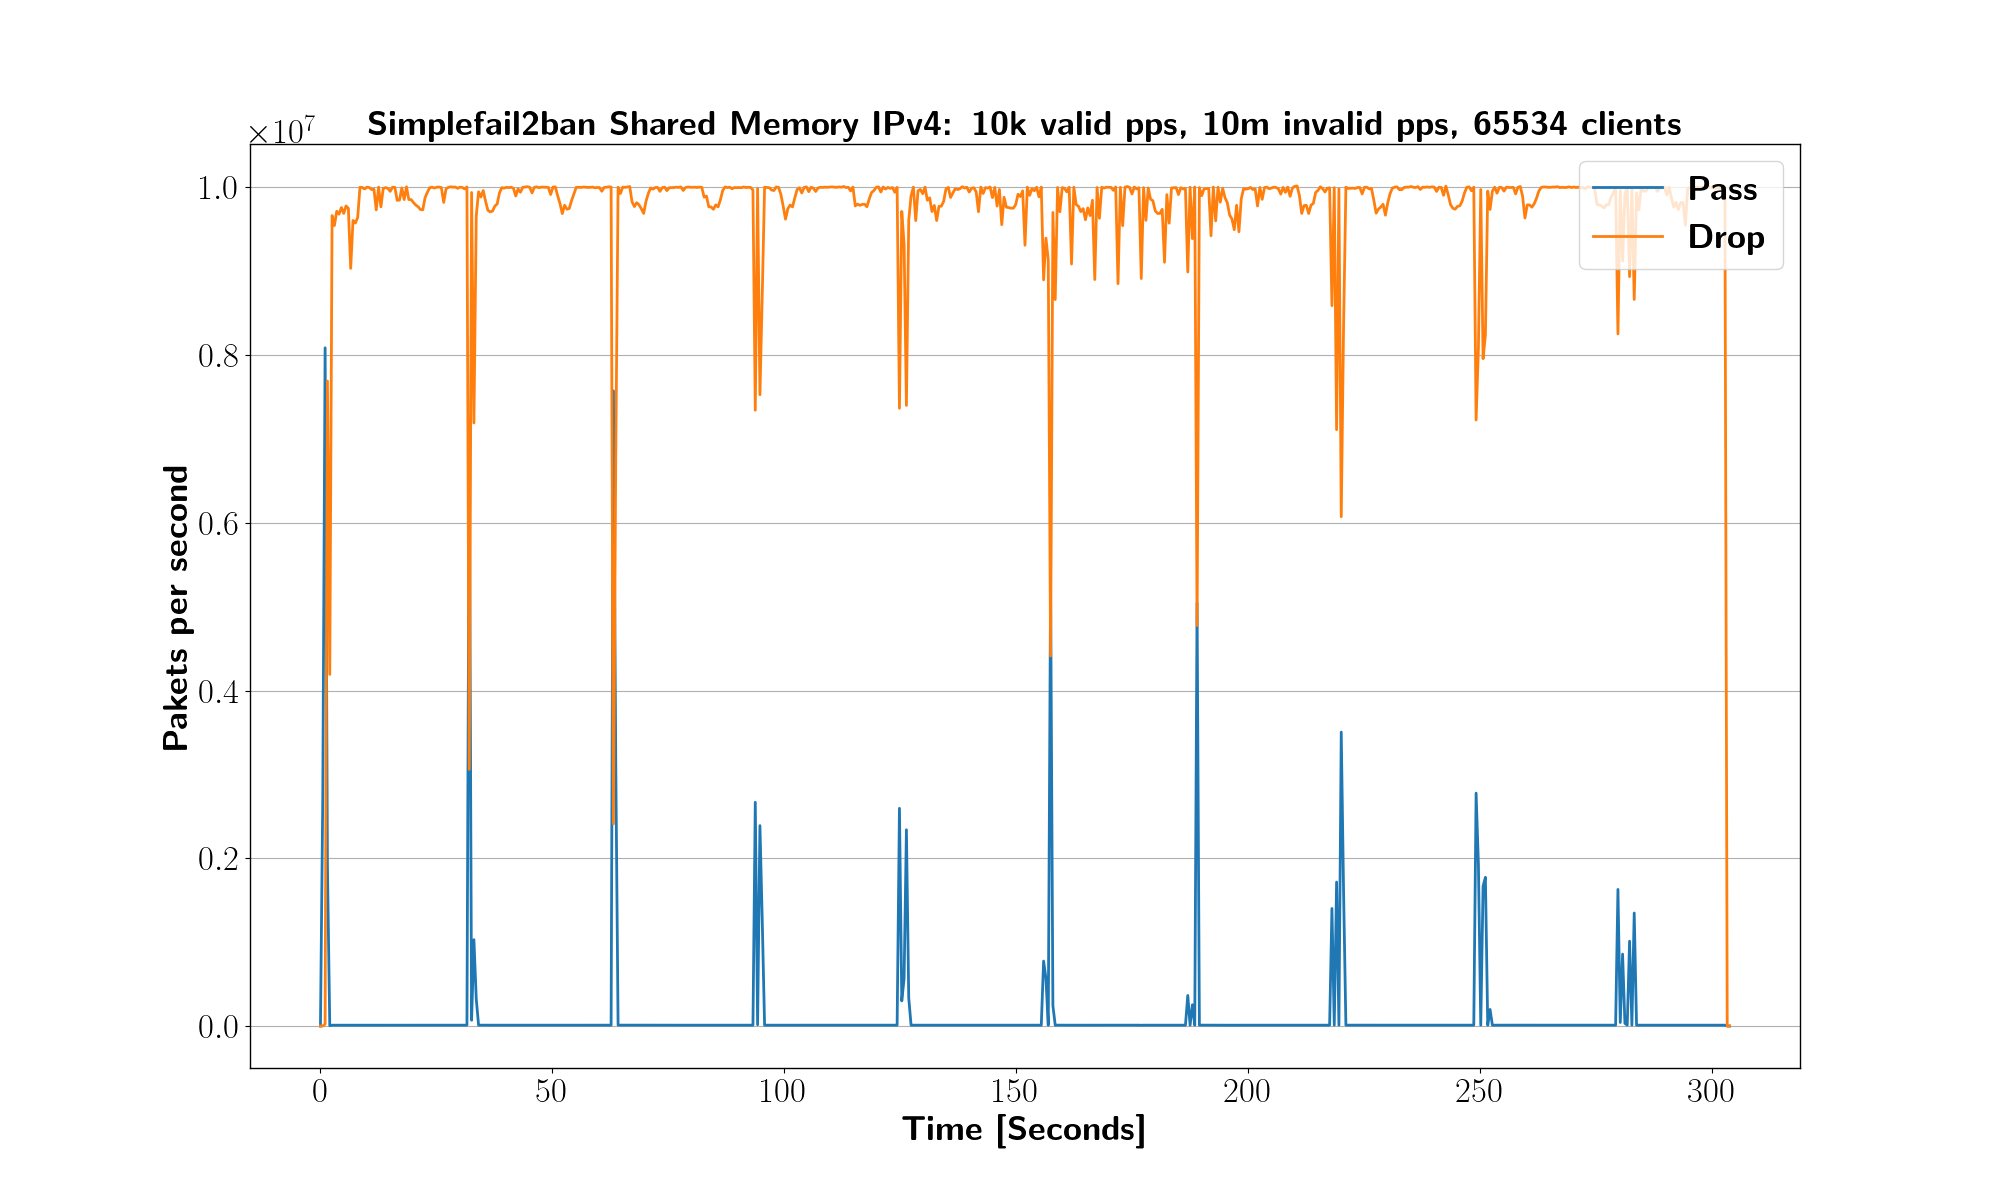
\includegraphics[width=1.2\textwidth]{images/simplefail2ban_shm_ipv4_v10k_iv10m_c65534.png}}
	\end{tabular}
	\begin{tabular}{lllll}
		\toprule
		\textbf{Total packets [$10^6$]} & \textbf{Packets dropped [$10^6$]} & \textbf{Relative drop [\%]} & \textbf{Log messages [$10^6$]} & \textbf{CPU [seconds]} \\ \midrule 
		2991.48 & 2948.51 & 96.72 & 7.69 & 25.59 \\
		\bottomrule
	\end{tabular}
	\caption[Simplefail2ban, Shared Memory, IPv4, 10m \ac{PPS}]{Some text}
\end{figure}

\begin{figure}[p]
	\label{fig:simplefail2ban:shm:ip6:100k}
	\centering
	\scriptsize
	\begin{tabular}{c}
    	\centerline{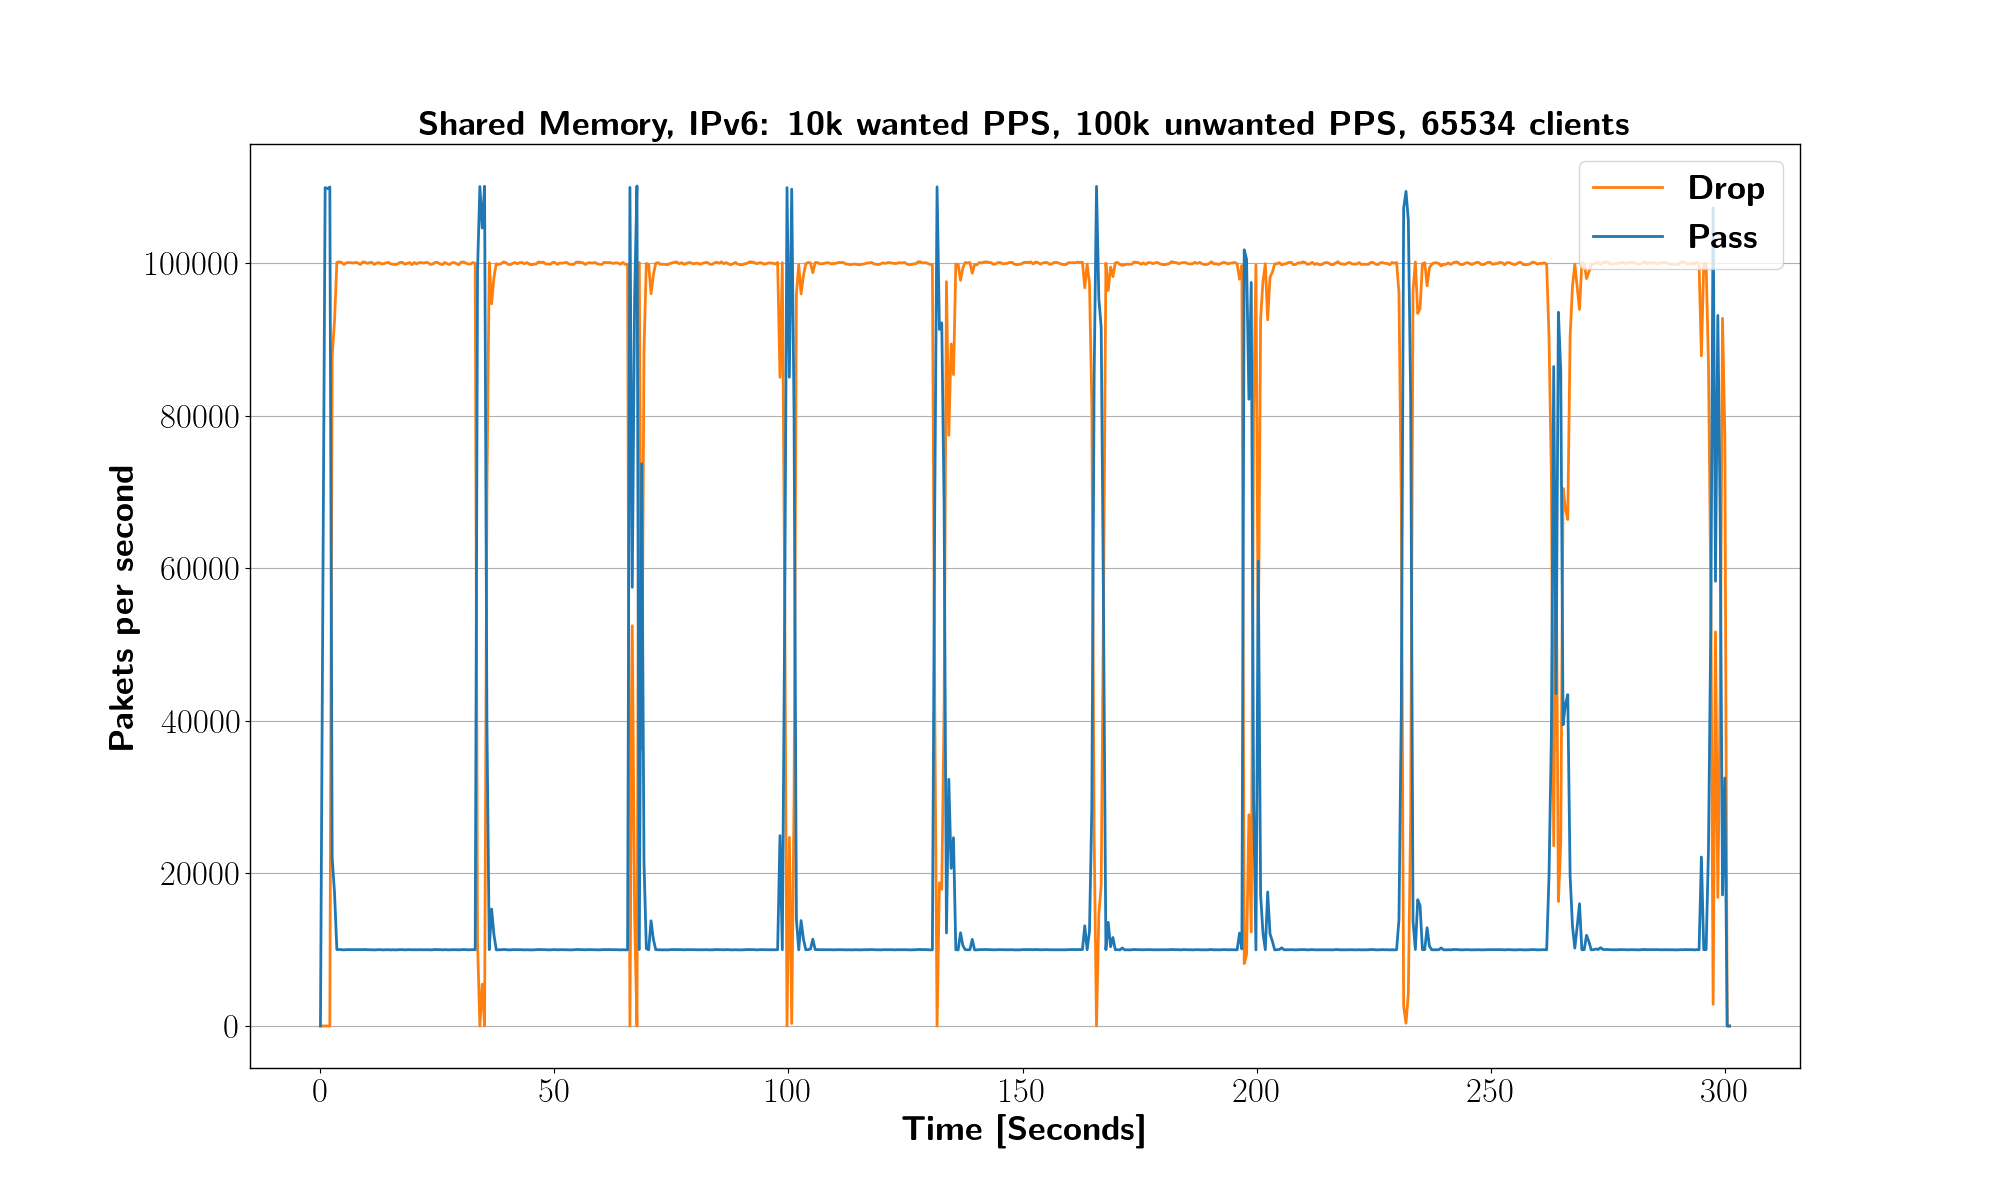
\includegraphics[width=1.2\textwidth]{images/simplefail2ban_shm_ipv6_v10k_iv100k_c65534.png}}
	\end{tabular}
	\begin{tabular}{lllll}
		\toprule
		\textbf{Total packets [$10^6$]} & \textbf{Packets dropped [$10^6$]} & \textbf{Relative drop [\%]} & \textbf{Log messages [$10^6$]} & \textbf{CPU [seconds]} \\ \midrule 
		33 & 27.95 & 99.67 & 2.05 & 15.55 \\
		\bottomrule
	\end{tabular}
	\caption[Simplefail2ban, Shared Memory, IPv6, 100k \ac{PPS}]{Some text}
\end{figure}

\begin{figure}[p]
	\label{fig:simplefail2ban:shm:ip6:1m}
	\centering
	\scriptsize
	\begin{tabular}{c}
    	\centerline{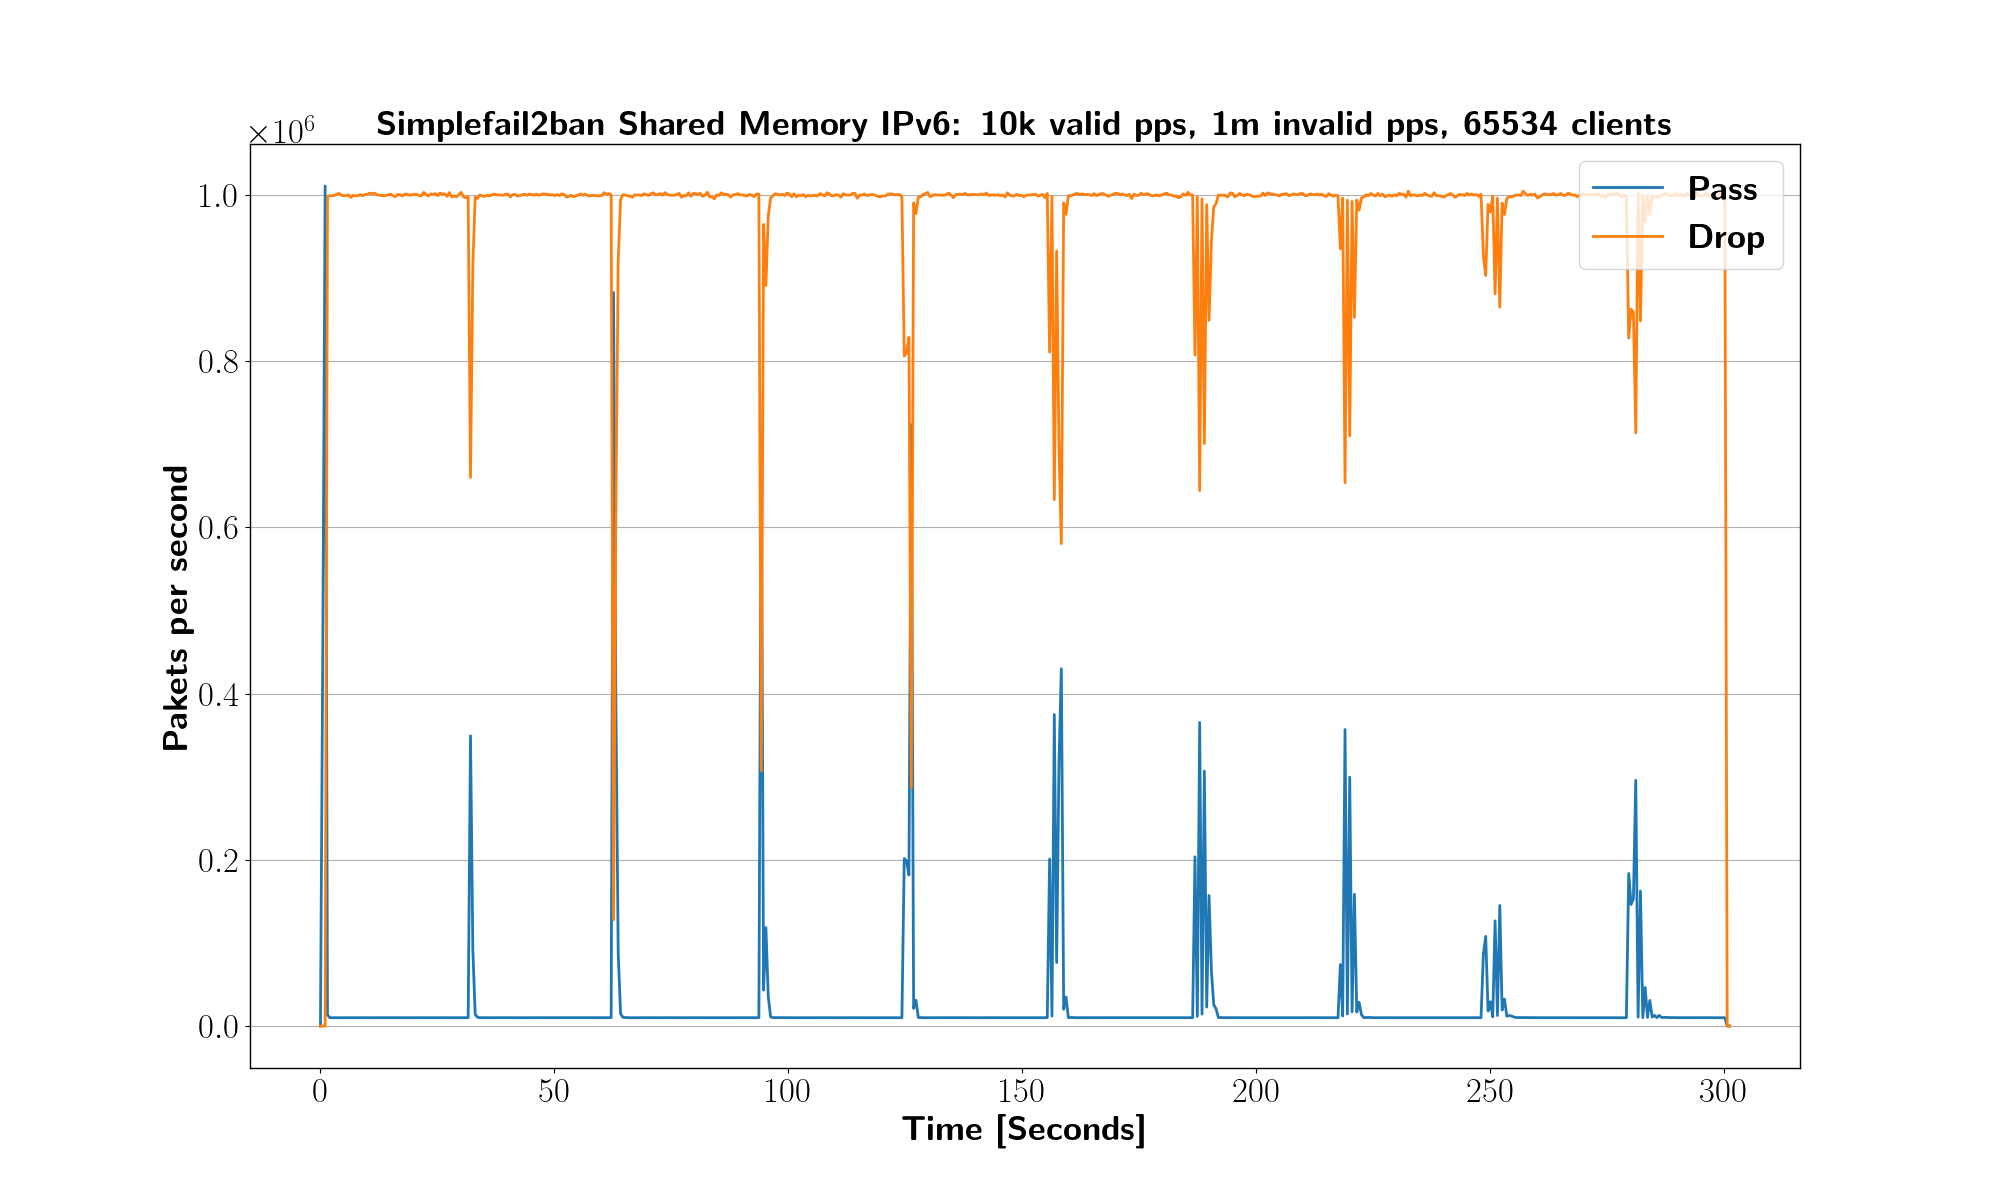
\includegraphics[width=1.2\textwidth]{images/simplefail2ban_shm_ipv6_v10k_iv1m_c65534.png}}
	\end{tabular}
	\begin{tabular}{lllll}
		\toprule
		\textbf{Total packets [$10^6$]} & \textbf{Packets dropped [$10^6$]} & \textbf{Relative drop [\%]} & \textbf{Log messages [$10^6$]} & \textbf{CPU [seconds]} \\ \midrule 
		303 & 294.77 & 98.9 & 4.39 & 17.46 \\
		\bottomrule
	\end{tabular}
	\caption[Simplefail2ban, Shared Memory, IPv6, 1m \ac{PPS}]{Some text}
\end{figure}

\begin{figure}[p]
	\label{fig:simplefail2ban:shm:ip6:10m}
	\centering
	\scriptsize
	\begin{tabular}{c}
    	\centerline{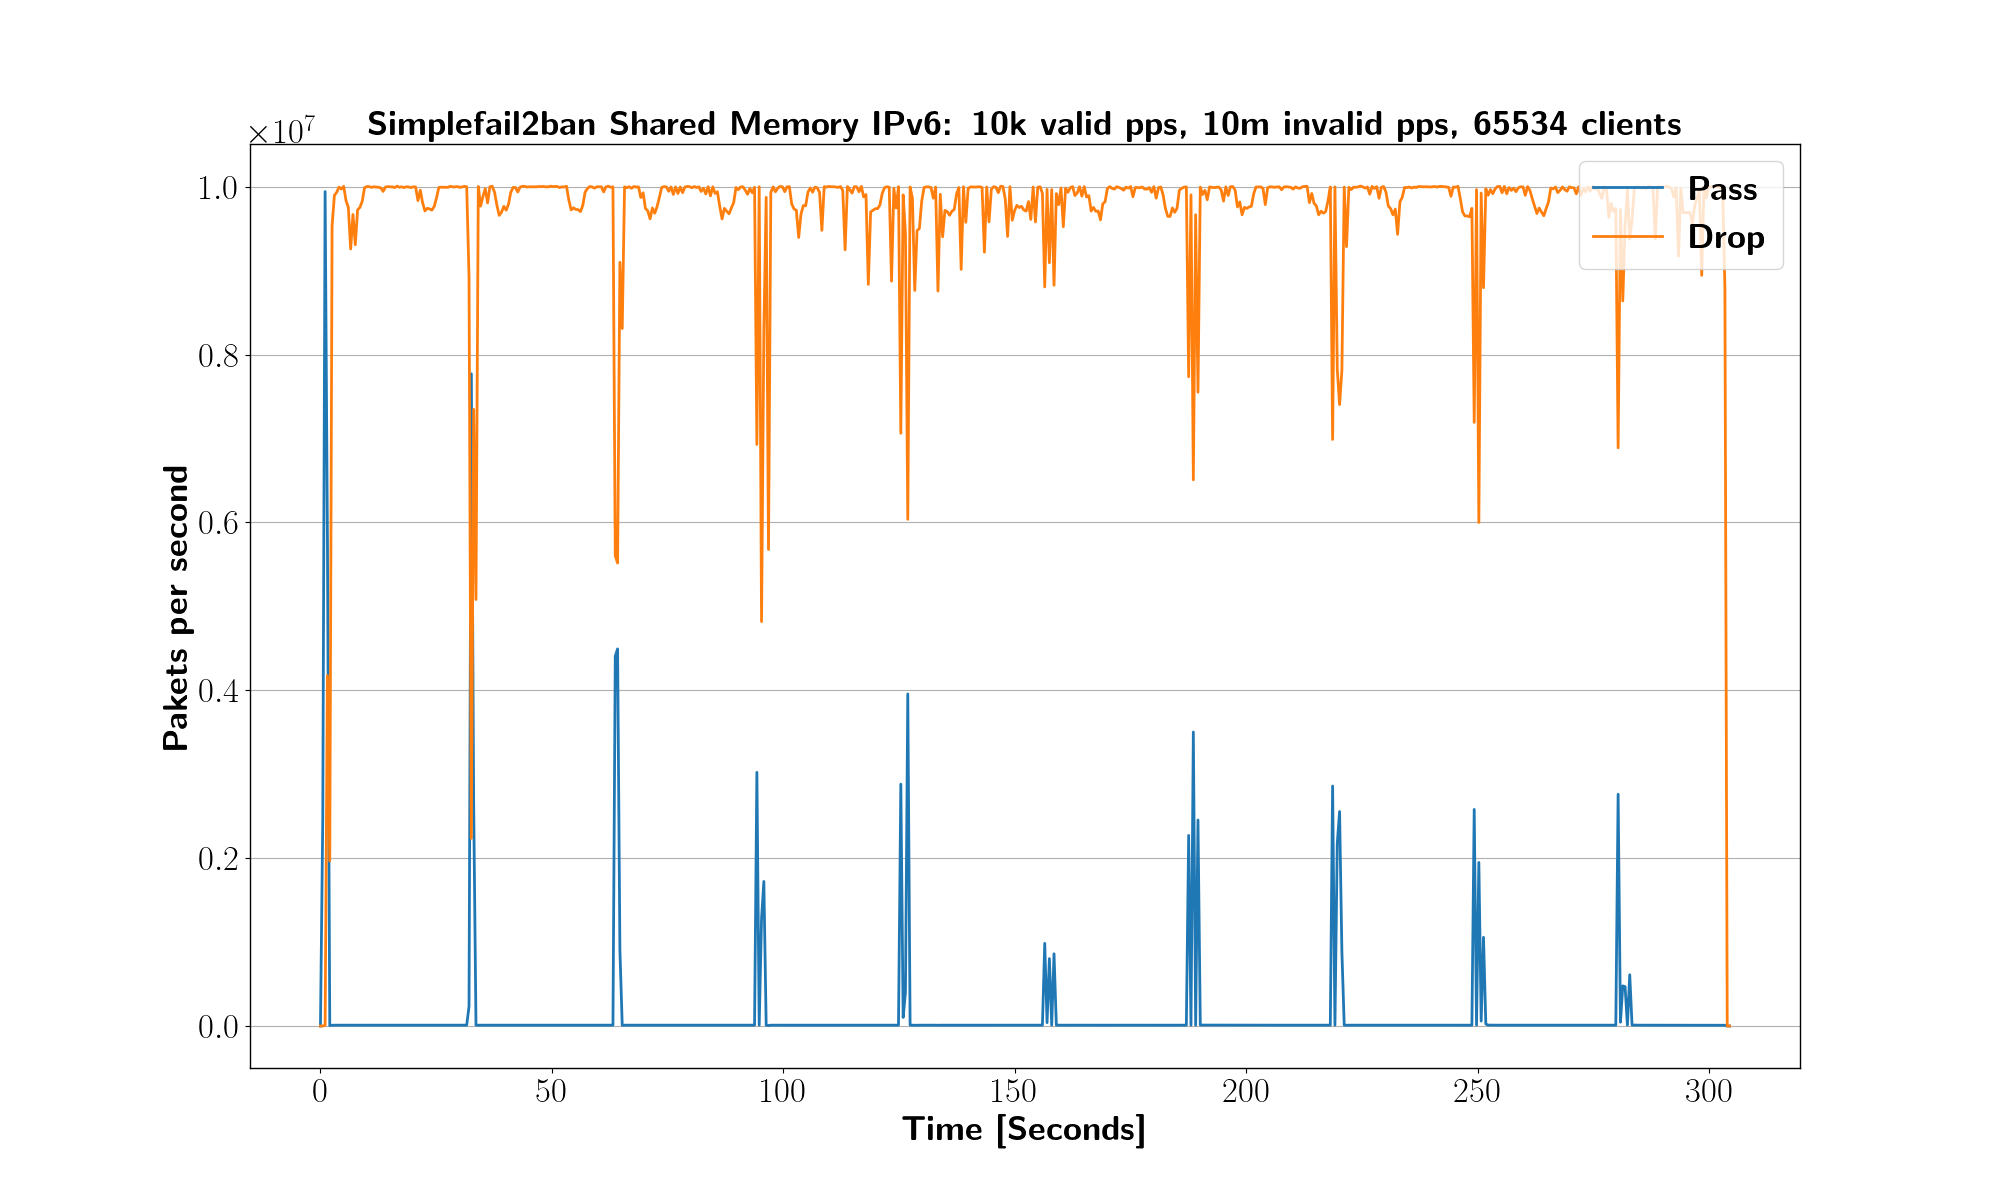
\includegraphics[width=1.2\textwidth]{images/simplefail2ban_shm_ipv6_v10k_iv10m_c65534.png}}
	\end{tabular}
	\begin{tabular}{lllll}
		\toprule
		\textbf{Total packets [$10^6$]} & \textbf{Packets dropped [$10^6$]} & \textbf{Relative drop [\%]} & \textbf{Log messages [$10^6$]} & \textbf{CPU [seconds]} \\ \midrule 
		2991.93 & 2947.1 & 98.66 & 8.88 & 32.36 \\
		\bottomrule
	\end{tabular}
	\caption[Simplefail2ban, Shared Memory, IPv6, 10m \ac{PPS}]{Some text}
\end{figure}

\begin{figure}[p]
	\label{fig:simplefail2ban:shm:ip46:100k}
	\centering
	\scriptsize
	\begin{tabular}{c}
    	\centerline{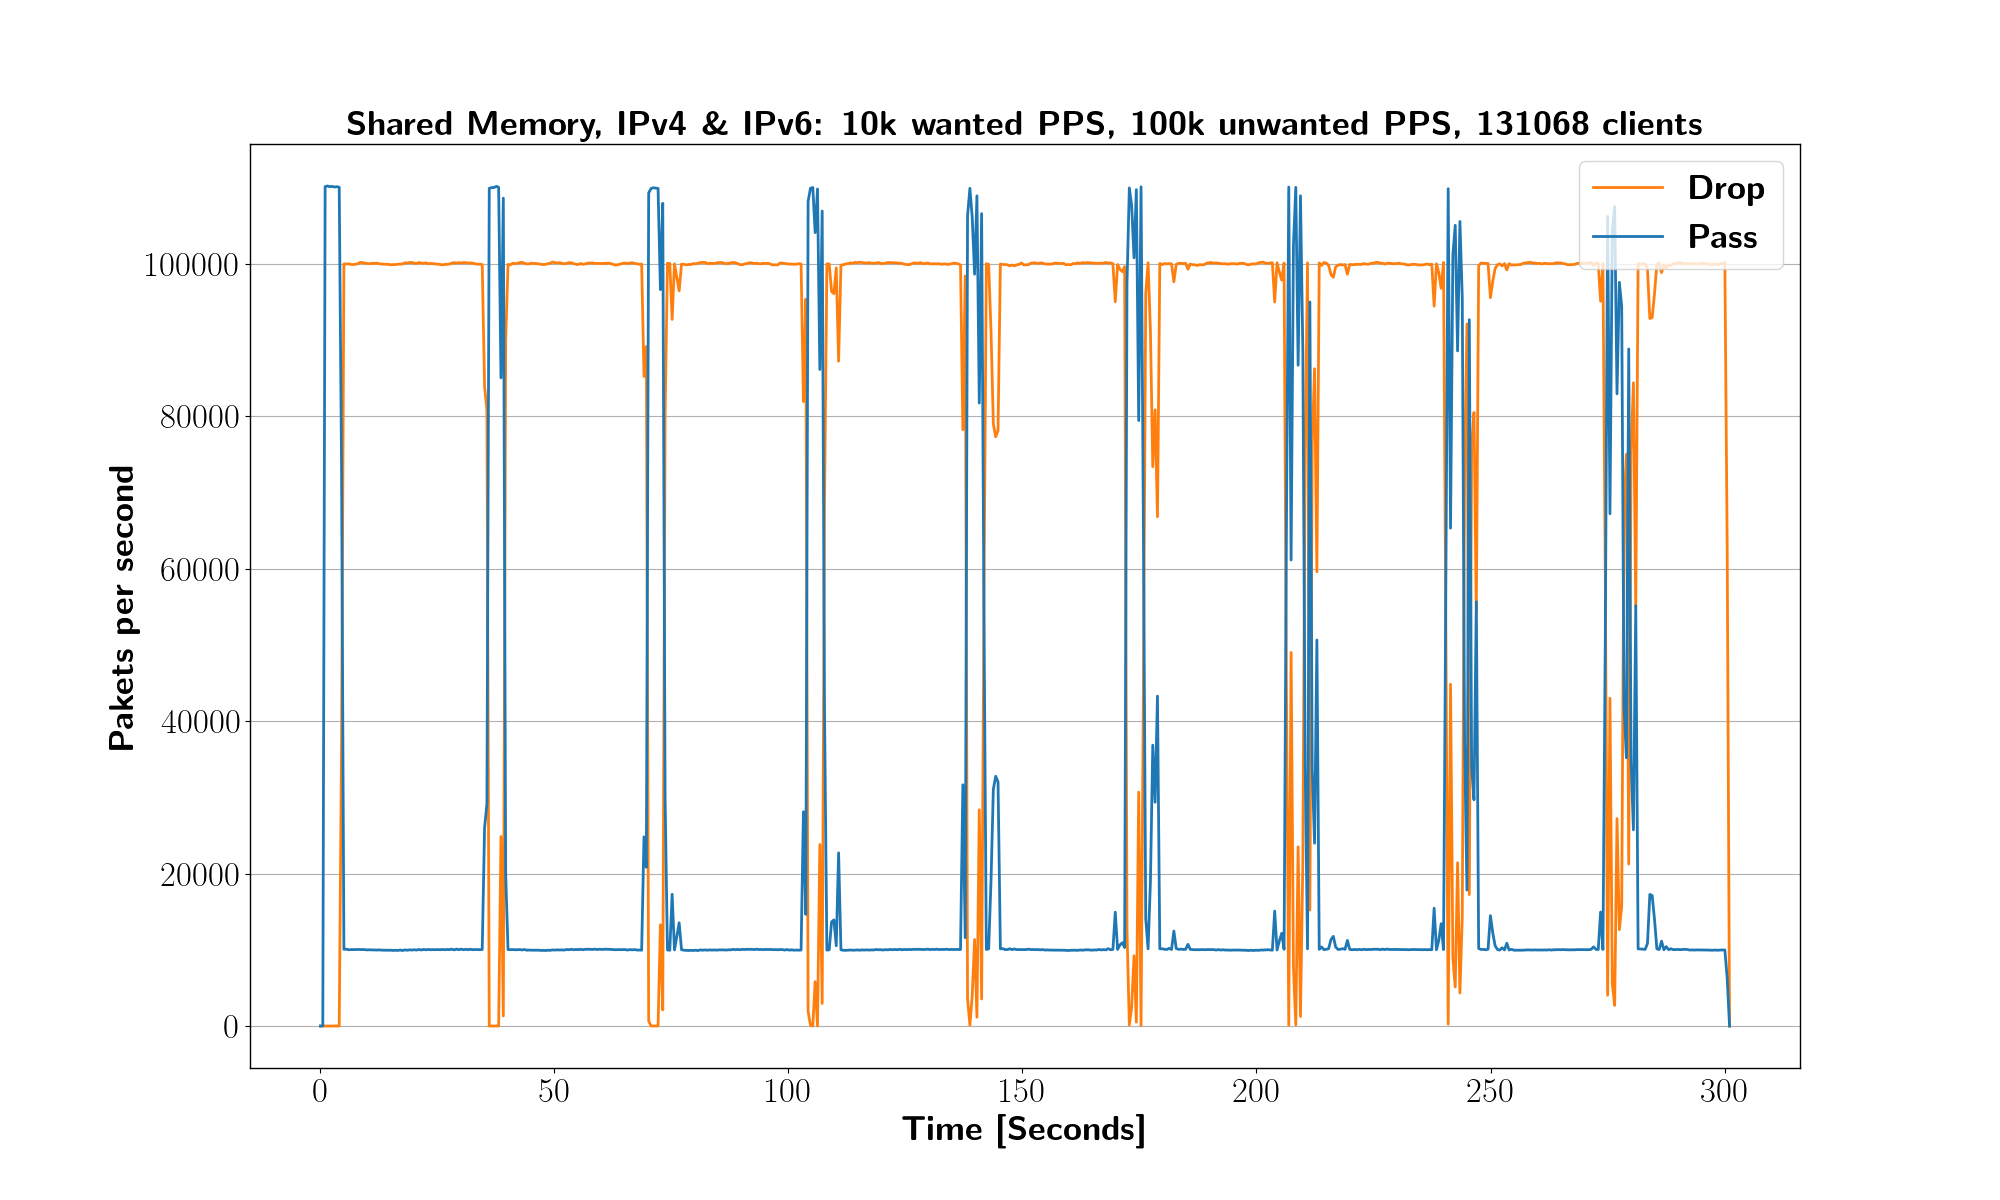
\includegraphics[width=1.2\textwidth]{images/simplefail2ban_shm_ipv46_v10k_iv100k_c131068.png}}
	\end{tabular}
	\begin{tabular}{lllll}
		\toprule
		\textbf{Total packets [$10^6$]} & \textbf{Packets dropped [$10^6$]} & \textbf{Relative drop [\%]} & \textbf{Log messages [$10^6$]} & \textbf{CPU [seconds]} \\ \midrule 
		33 & 26.45 & 99.95 & 3.55 & 26.35 \\
		\bottomrule
	\end{tabular}
	\caption[Simplefail2ban, Shared Memory, IPv4 \& IPv6, 100k \ac{PPS}]{Some text}
\end{figure}

\begin{figure}[p]
	\label{fig:simplefail2ban:shm:ip46:1m}
	\centering
	\scriptsize
	\begin{tabular}{c}
    	\centerline{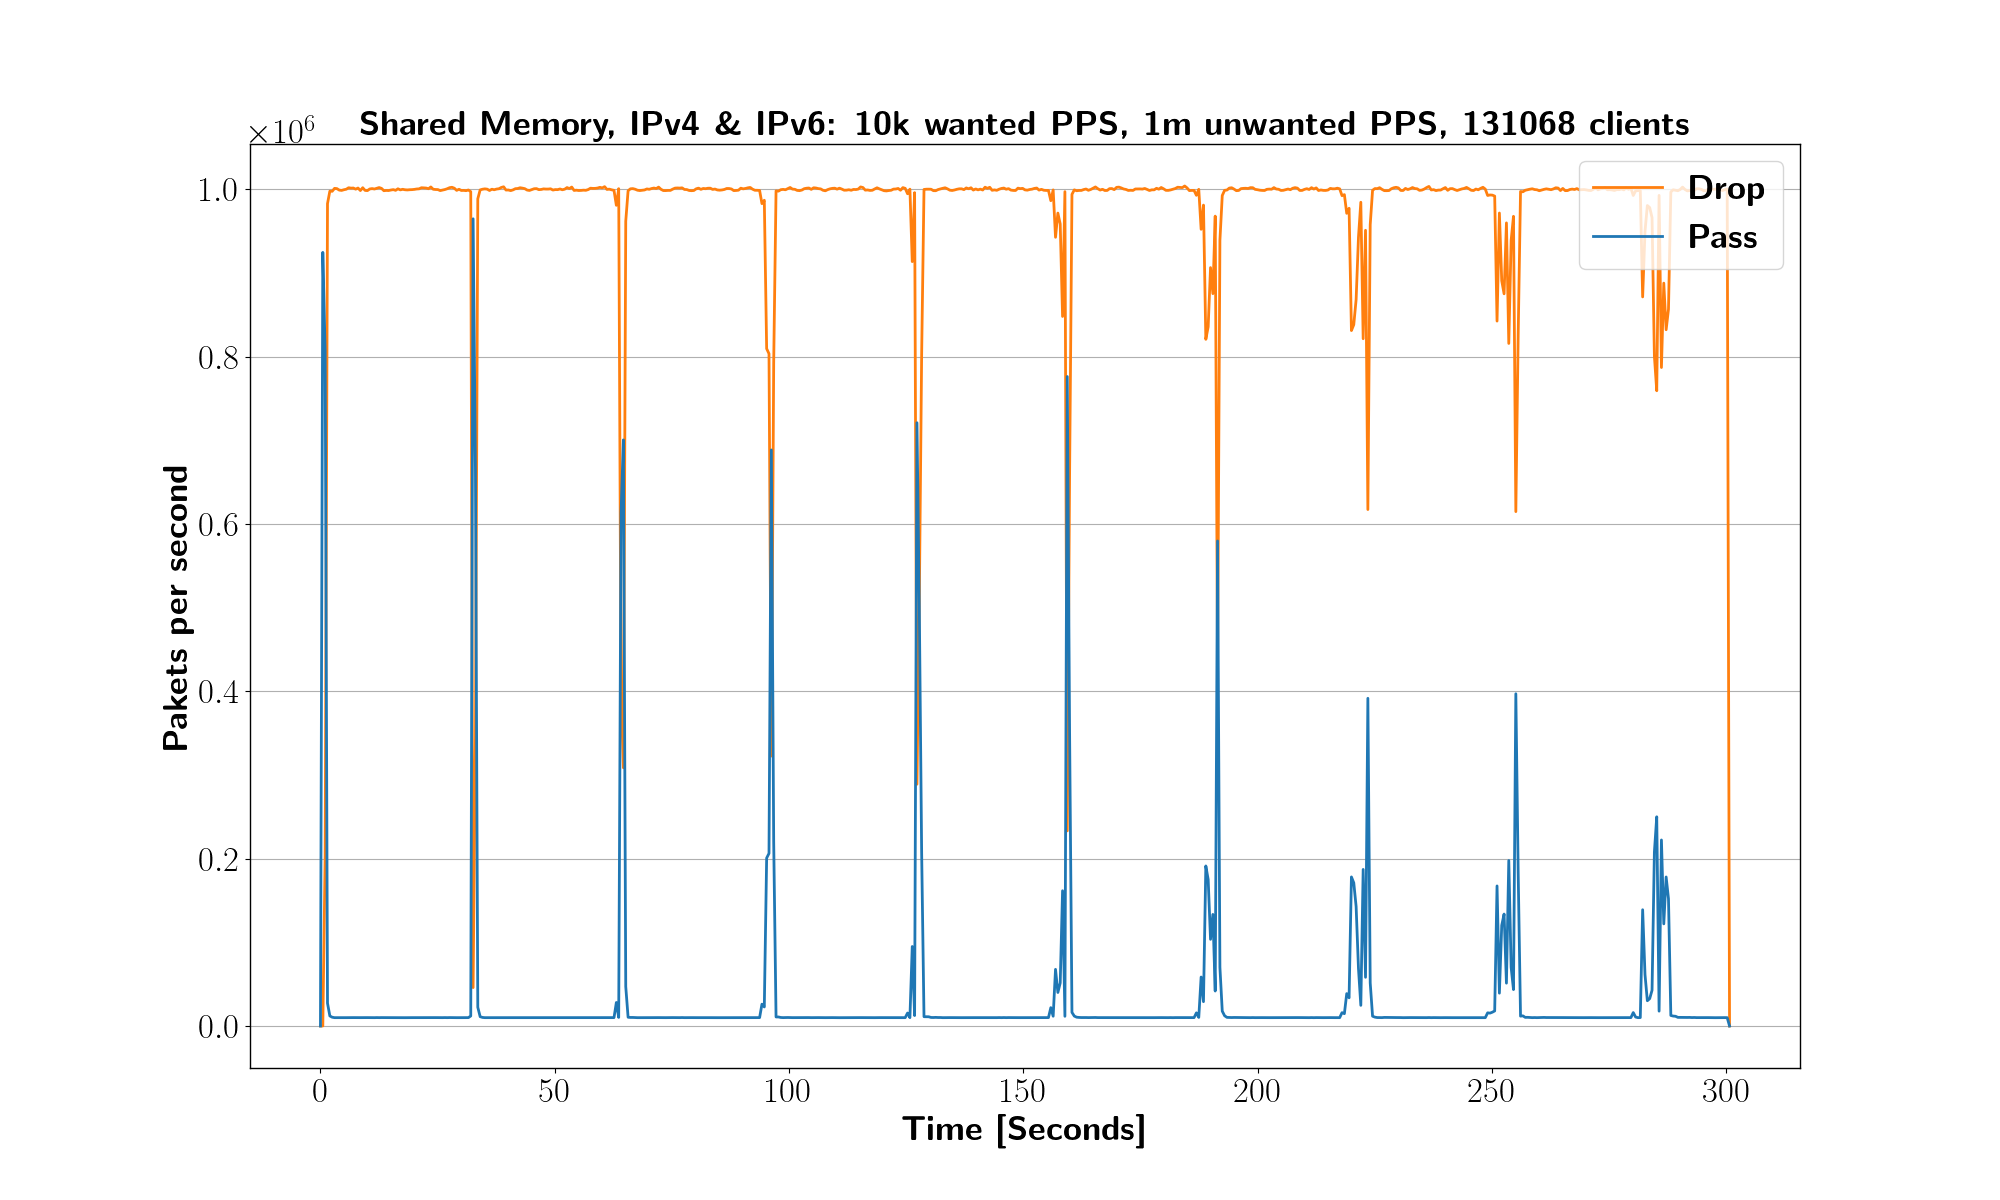
\includegraphics[width=1.2\textwidth]{images/simplefail2ban_shm_ipv46_v10k_iv1m_c131068.png}}
	\end{tabular}
	\begin{tabular}{lllll}
		\toprule
		\textbf{Total packets [$10^6$]} & \textbf{Packets dropped [$10^6$]} & \textbf{Relative drop [\%]} & \textbf{Log messages [$10^6$]} & \textbf{CPU [seconds]} \\ \midrule 
		303 & 293.13 & 99 & 5.95 & 27.66 \\
		\bottomrule
	\end{tabular}
	\caption[Simplefail2ban, Shared Memory, IPv4 \& IPv6, 1m \ac{PPS}]{Some text}
\end{figure}

\begin{figure}[p]
	\label{fig:simplefail2ban:shm:ip46:10m}
	\centering
	\scriptsize
	\begin{tabular}{c}
    	\centerline{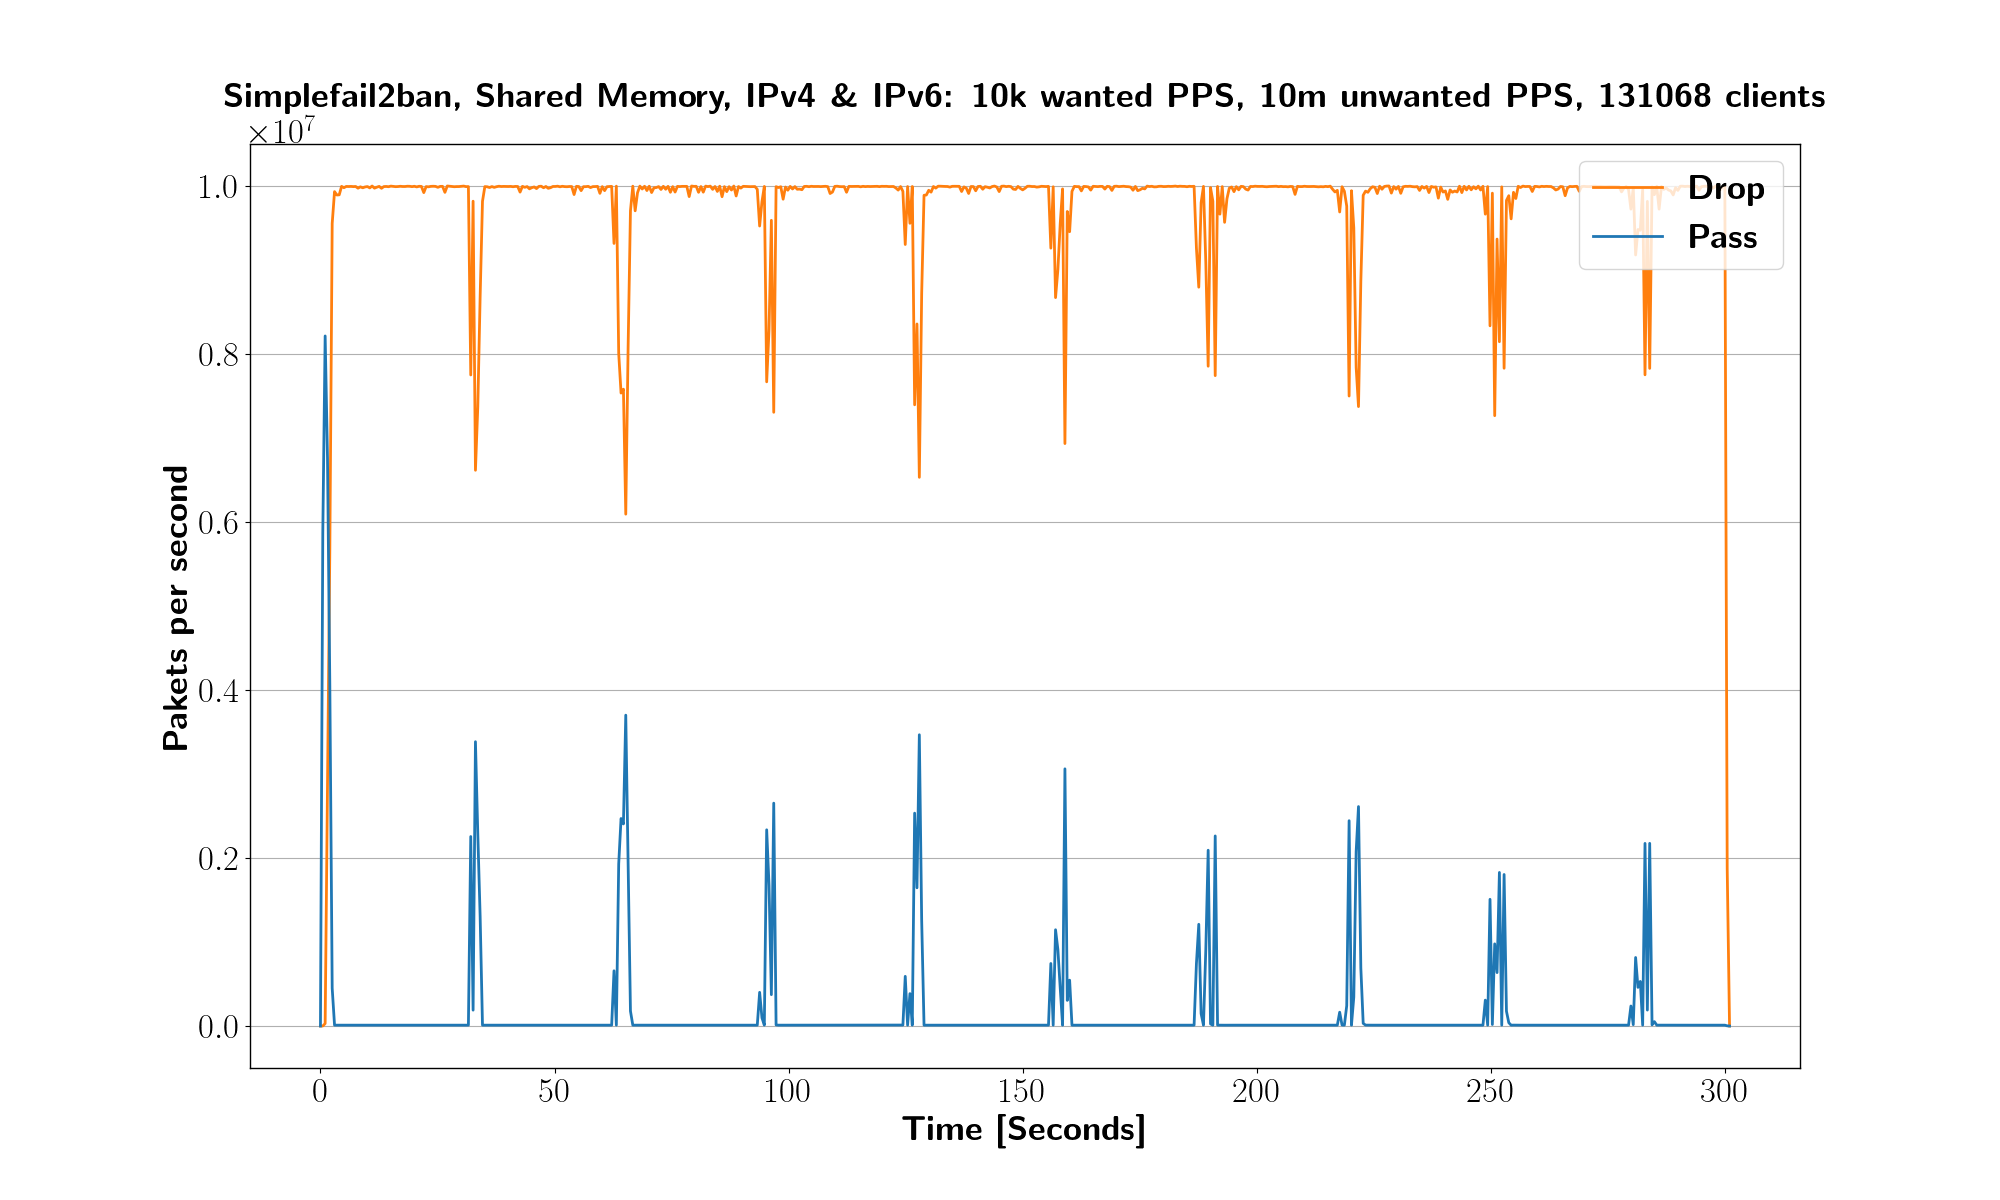
\includegraphics[width=1.2\textwidth]{images/simplefail2ban_shm_ipv46_v10k_iv10m_c131068.png}}
	\end{tabular}
	\begin{tabular}{lllll}
		\toprule
		\textbf{Total packets [$10^6$]} & \textbf{Packets dropped [$10^6$]} & \textbf{Relative drop [\%]} & \textbf{Log messages [$10^6$]} & \textbf{CPU [seconds]} \\ \midrule 
		2992.44 & 2939.27 & 98.45 & 16.18 & 65.74 \\
		\bottomrule
	\end{tabular}
	\caption[Simplefail2ban, Shared Memory, IPv4 \& IPv6, 10m \ac{PPS}]{Some text}
\end{figure}

\begin{figure}[p]
	\label{fig:simplefail2ban:shm:ip46:30m}
	\centering
	\scriptsize
	\begin{tabular}{c}
    	\centerline{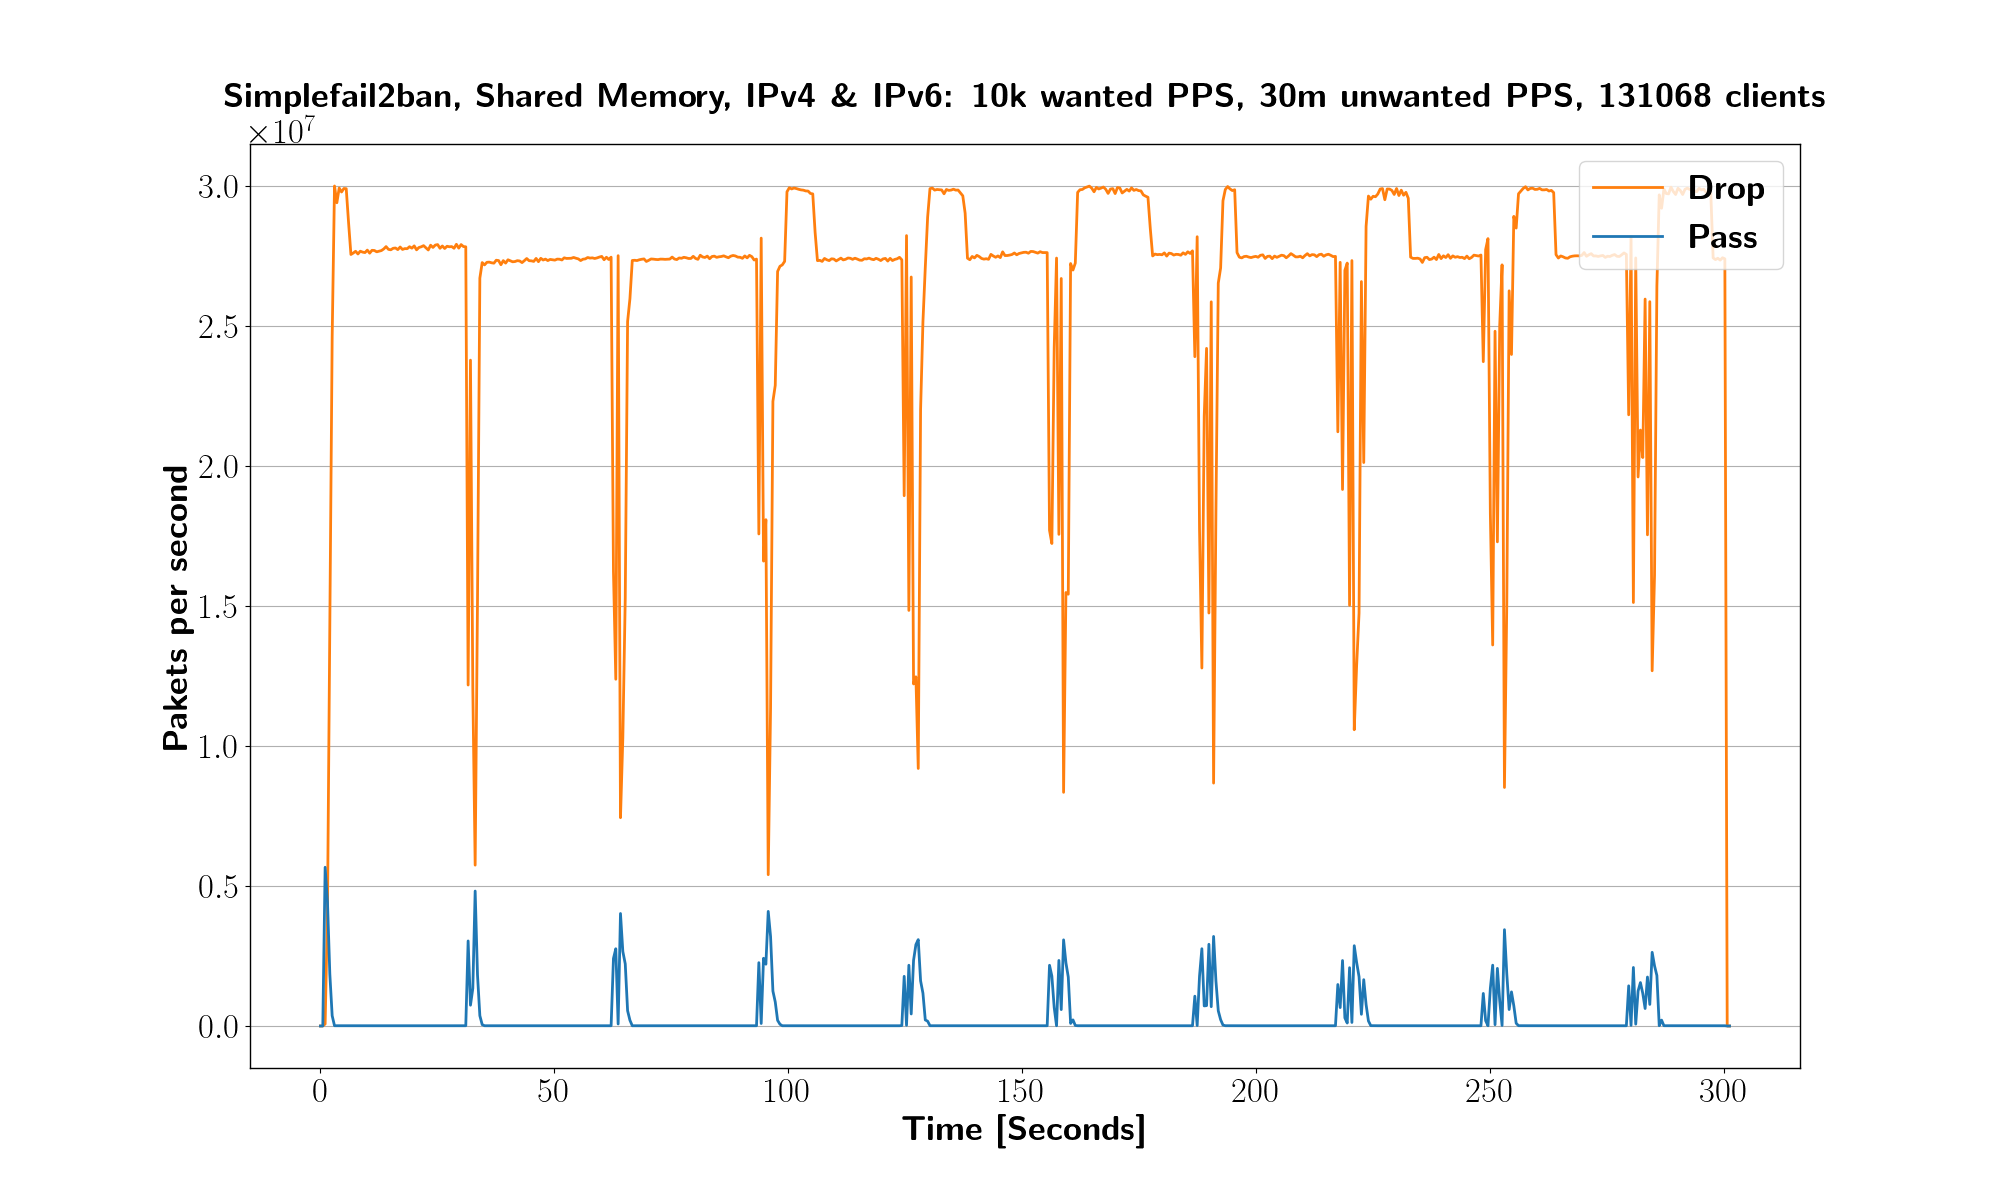
\includegraphics[width=1.2\textwidth]{images/simplefail2ban_shm_ipv46_v10k_iv30m_c131068.png}}
	\end{tabular}
	\begin{tabular}{lllll}
		\toprule
		\textbf{Total packets [$10^6$]} & \textbf{Packets dropped [$10^6$]} & \textbf{Relative drop [\%]} & \textbf{Log messages [$10^6$]} & \textbf{CPU [seconds]} \\ \midrule 
		8095.28 & 8017.72 & 99.13 & 21 & 76.23 \\
		\bottomrule
	\end{tabular}
	\caption[Simplefail2ban, Shared Memory, IPv4 \& IPv6, 30m \ac{PPS}]{Some text}
\end{figure}

\section{Shared Memory Feature Measurements}

\begin{figure}[p]
	\label{fig:simplefail2ban:shm:2r}
	\centering
	\scriptsize
	\begin{tabular}{c}
    	\centerline{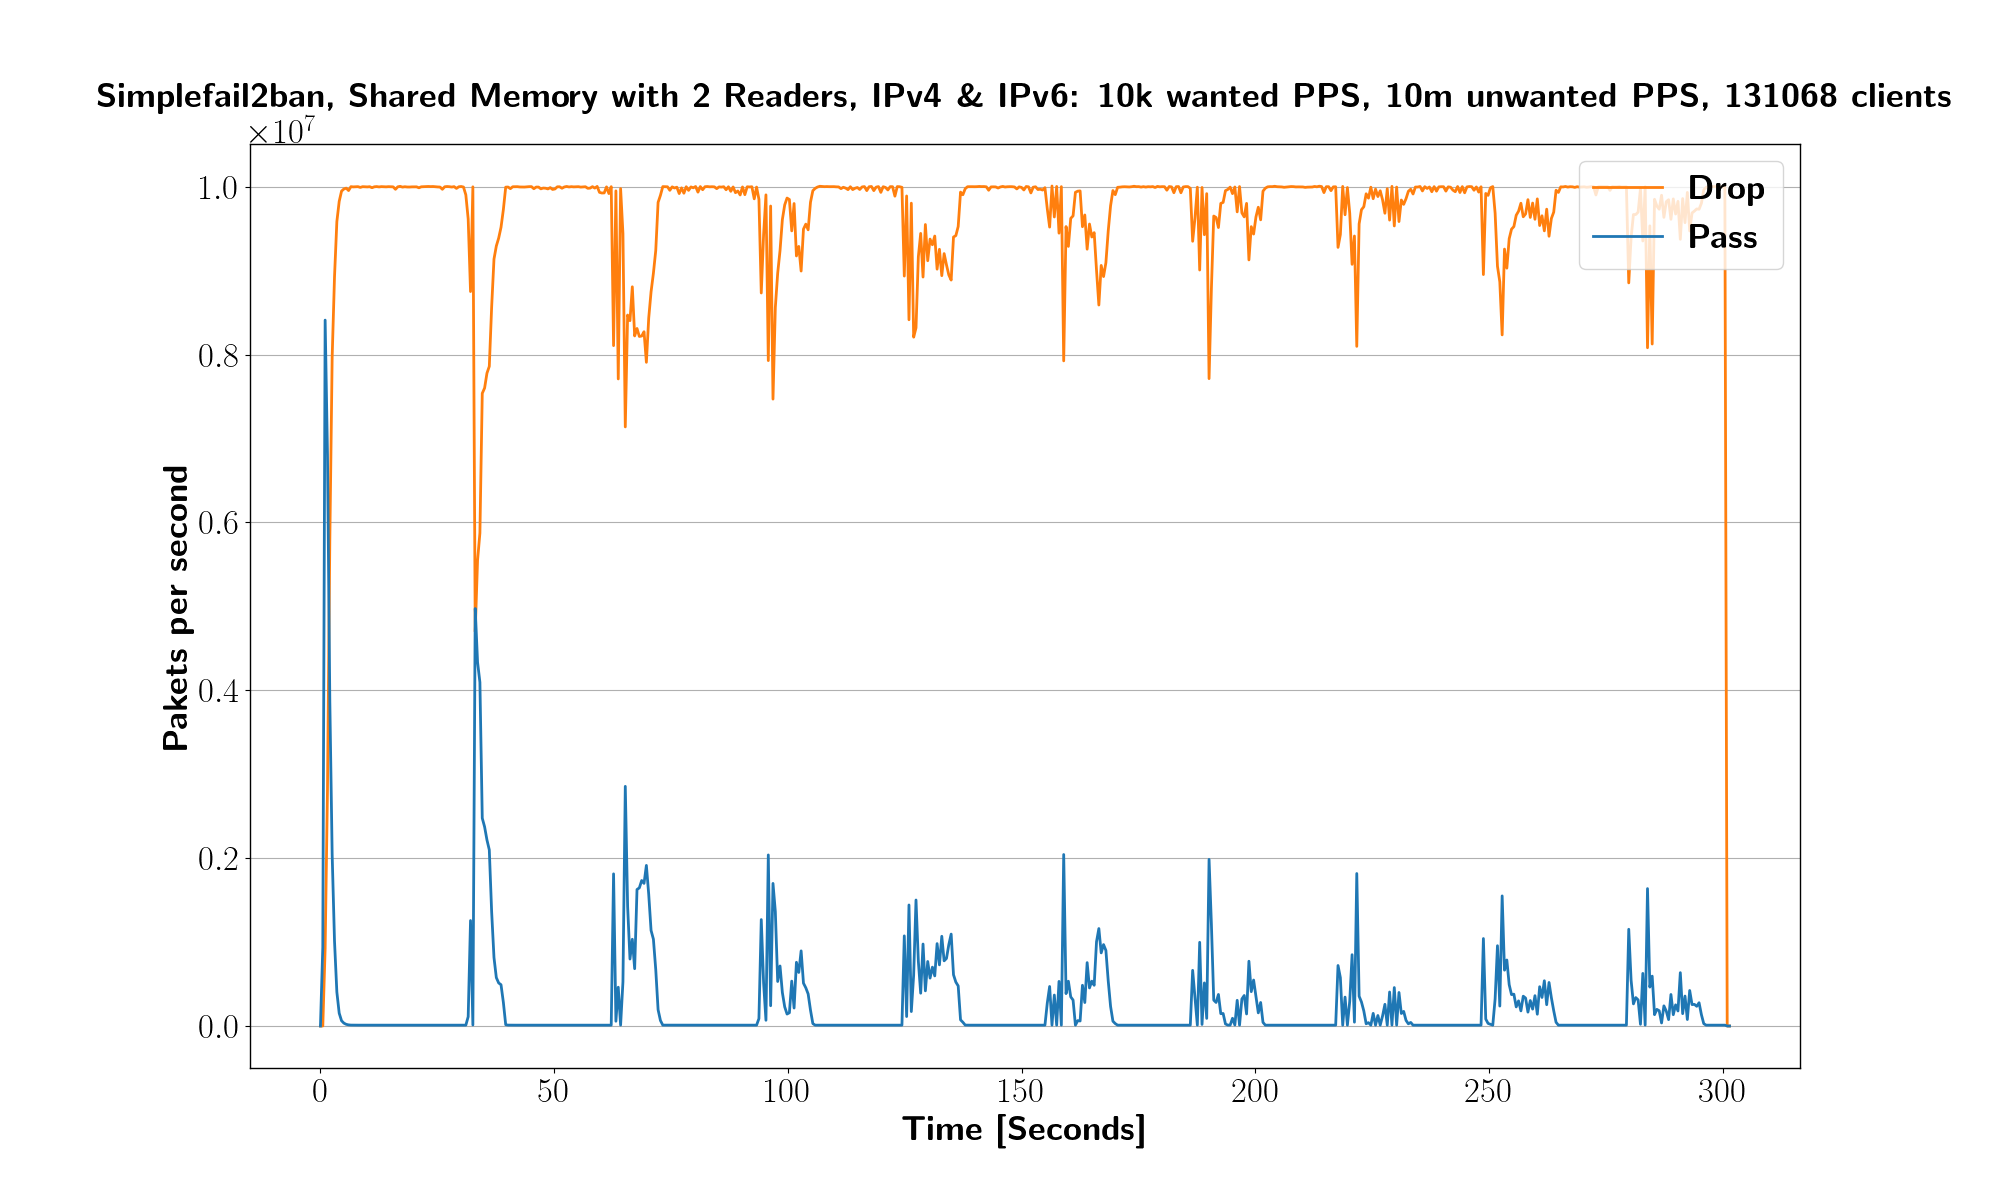
\includegraphics[width=1.2\textwidth]{images/simplefail2ban_shm_2r_ipv46_v10k_iv10m_c131068.png}}
	\end{tabular}
	\begin{tabular}{lllll}
		\toprule
		\textbf{Total packets [$10^6$]} & \textbf{Packets dropped [$10^6$]} & \textbf{Relative drop [\%]} & \textbf{Log messages [$10^6$]} & \textbf{CPU [seconds]} \\ \midrule 
		2989.66 & 2906.36 & 97.44 & 17.67 & 77.19 \\
		\bottomrule
	\end{tabular}
	\caption[Simplefail2ban, Shared Memory 2 Readers]{Some text}
\end{figure}

\begin{figure}[p]
	\label{fig:simplefail2ban:shm:or}
	\centering
	\scriptsize
	\begin{tabular}{c}
    	\centerline{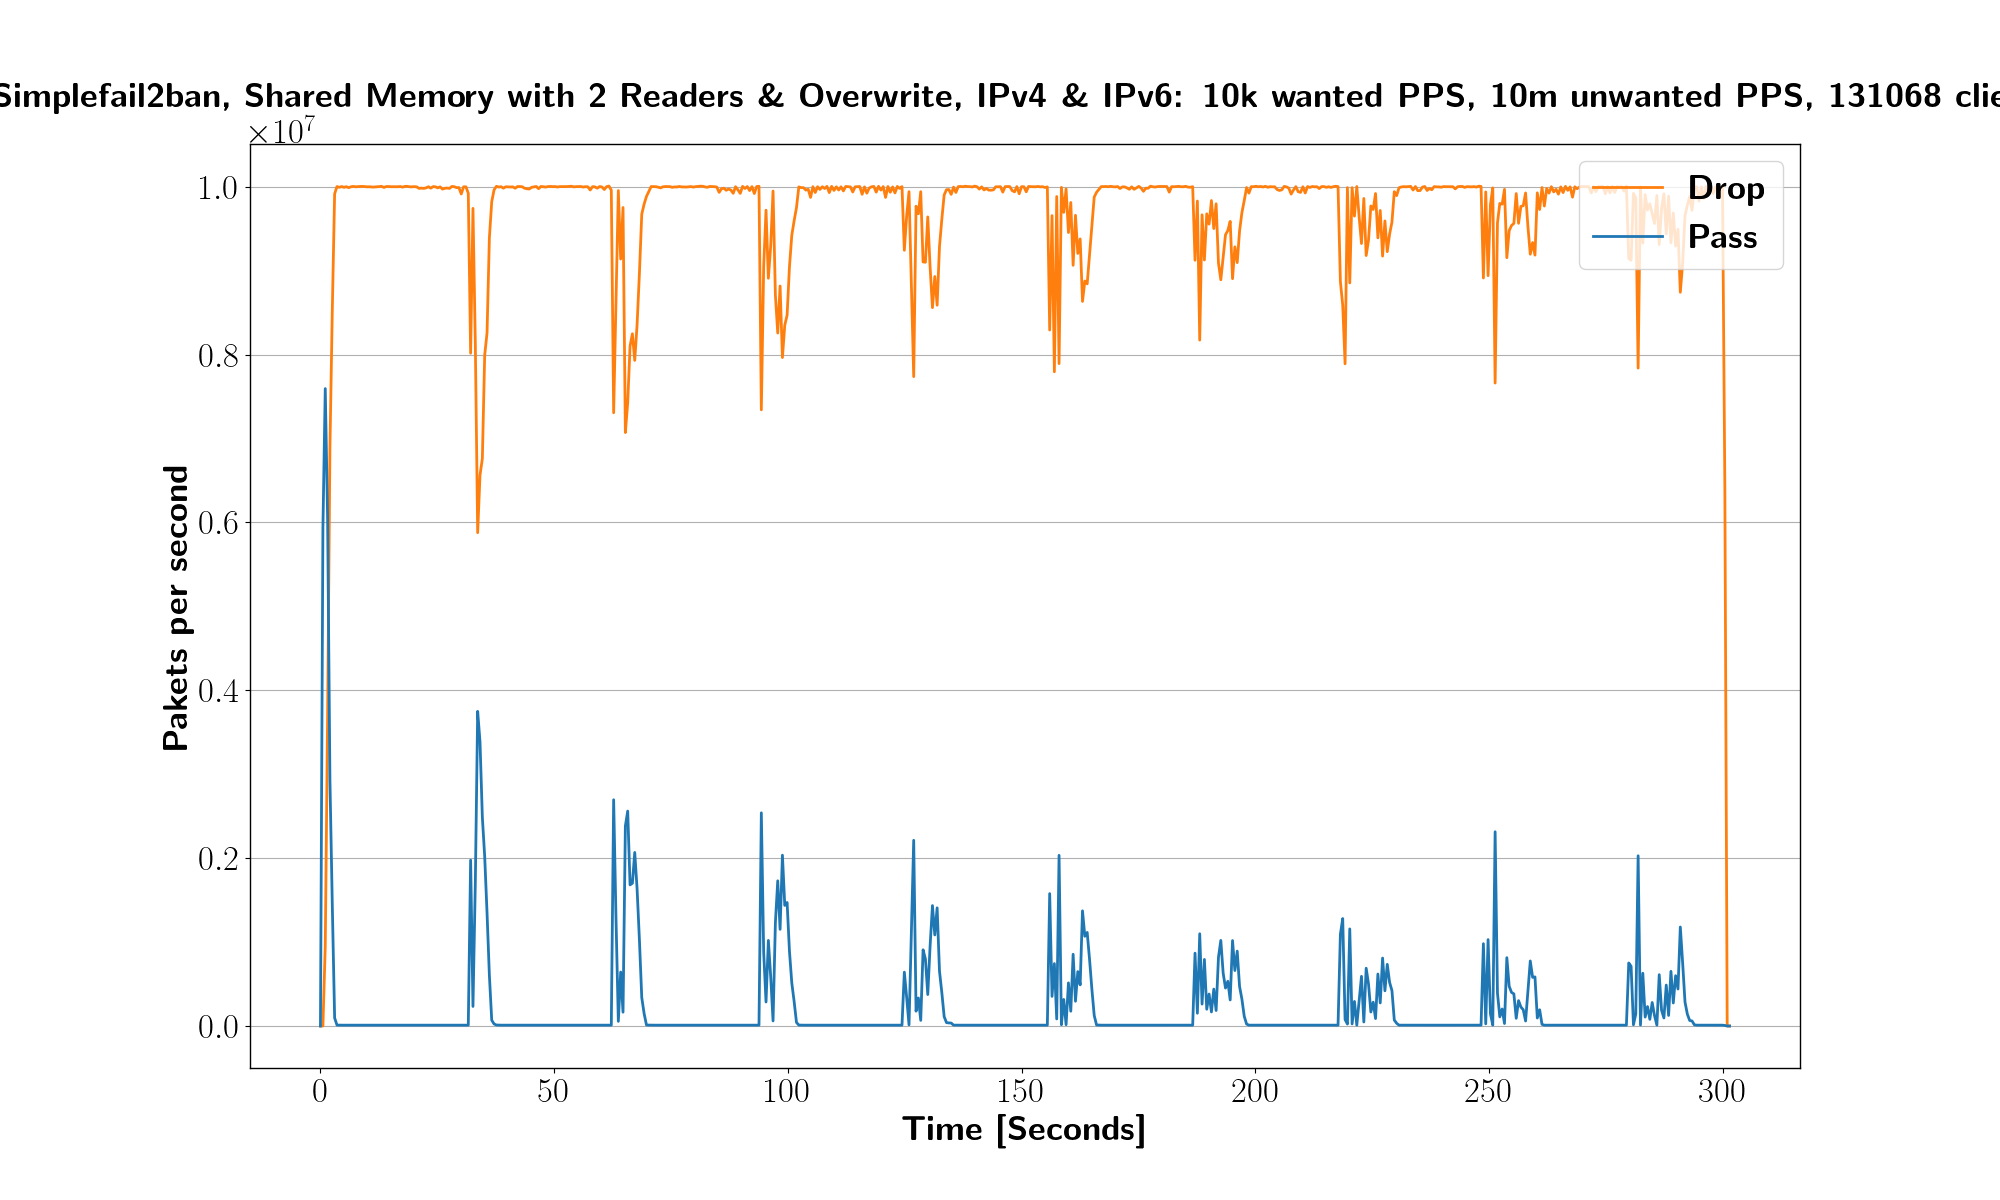
\includegraphics[width=1.2\textwidth]{images/simplefail2ban_shm_2r_or_ipv46_v10k_iv10m_c131068.png}}
	\end{tabular}
	\begin{tabular}{lllll}
		\toprule
		\textbf{Total packets [$10^6$]} & \textbf{Packets dropped [$10^6$]} & \textbf{Relative drop [\%]} & \textbf{Log messages [$10^6$]} & \textbf{CPU [seconds]} \\ \midrule 
		2988.9 & 2914.39 & 97.73 & 17.66 & 79.13 \\
		\bottomrule
	\end{tabular}
	\caption[Simplefail2ban, Shared Memory 2 Readers with Overwrite]{Some text}
\end{figure}

\begin{figure}[p]
	\label{fig:simplefail2ban:shm:ws}
	\centering
	\scriptsize
	\begin{tabular}{c}
    	\centerline{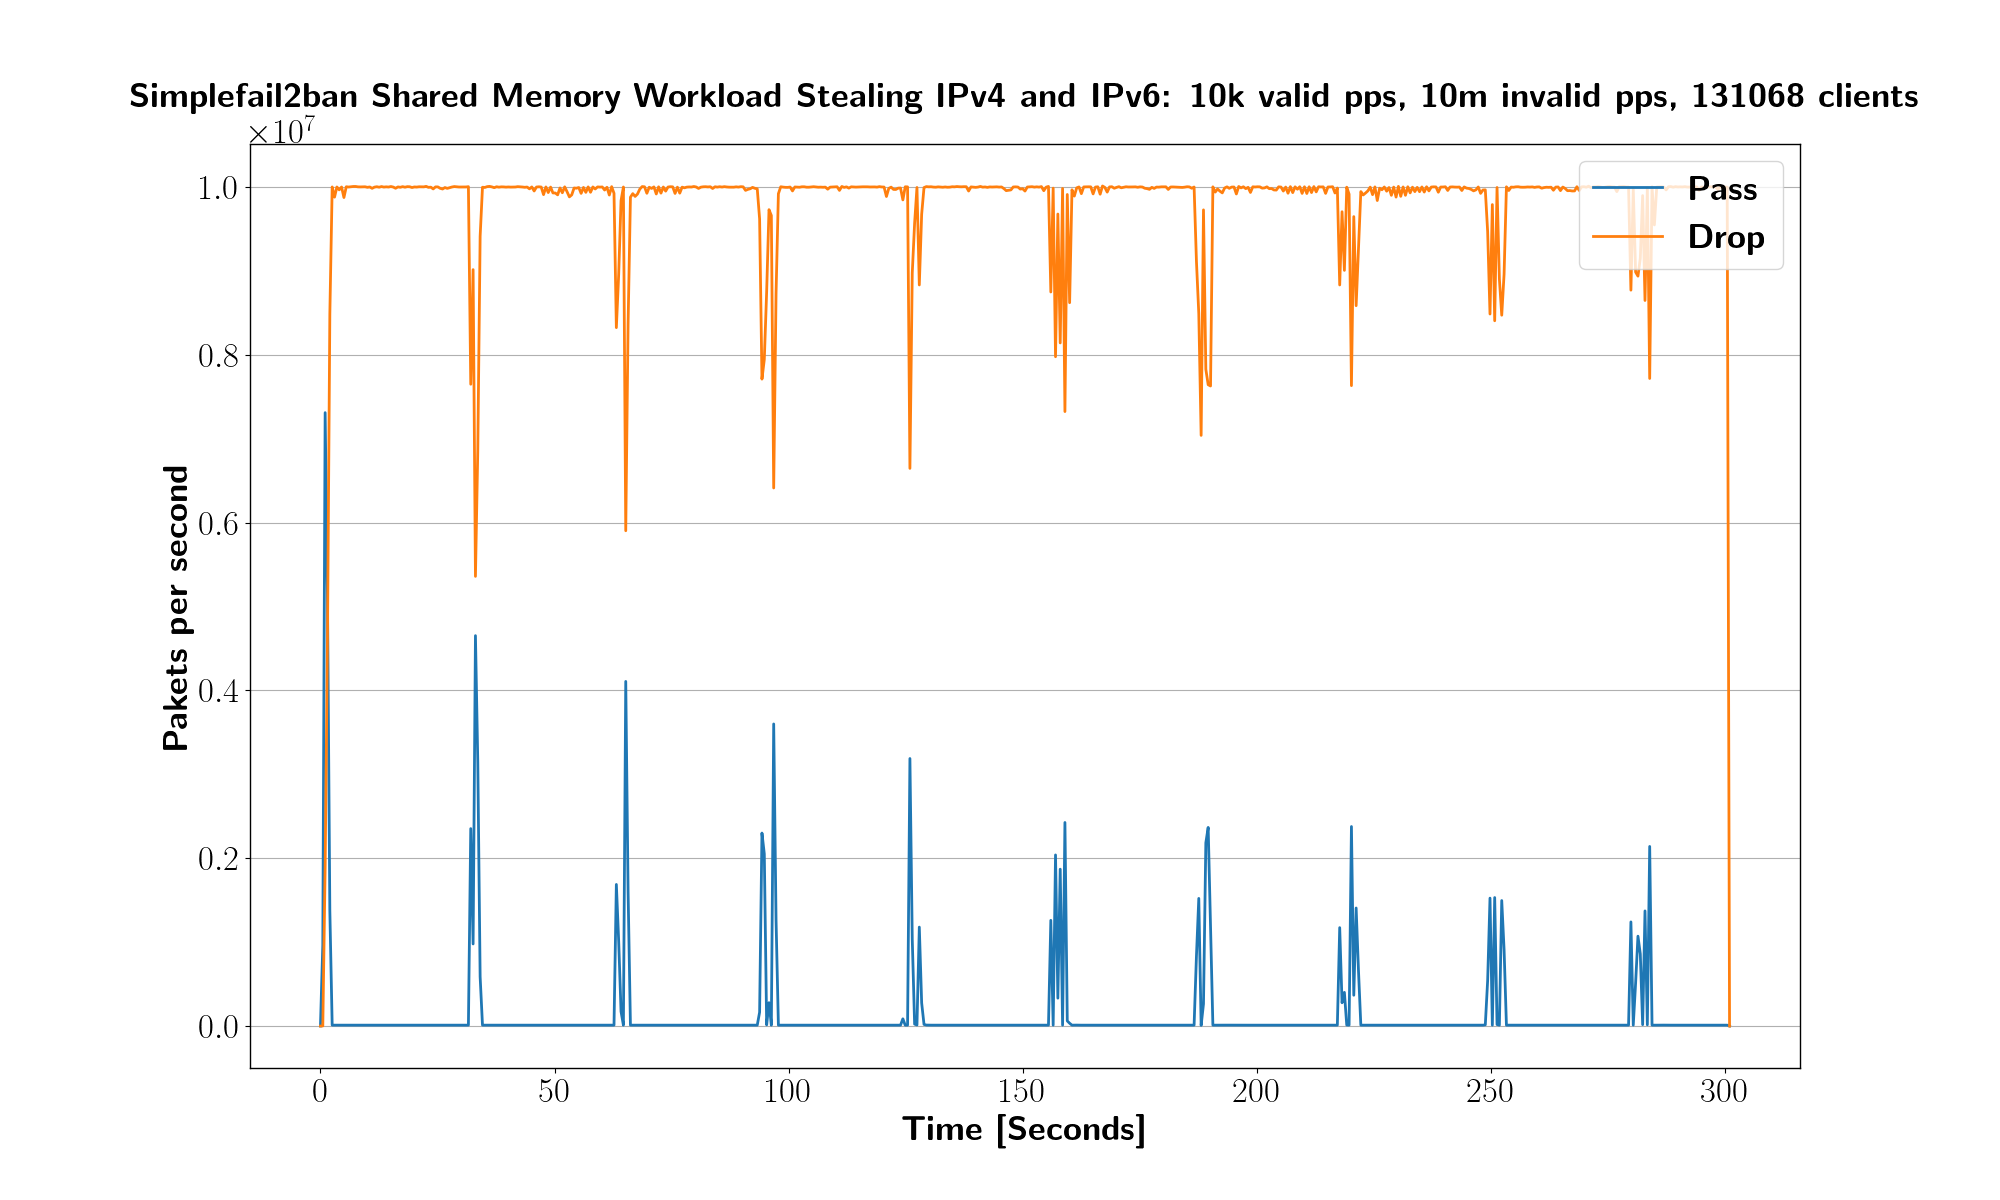
\includegraphics[width=1.2\textwidth]{images/simplefail2ban_shm_ws_ipv46_v10k_iv10m_c131068.png}}
	\end{tabular}
	\begin{tabular}{lllll}
		\toprule
		\textbf{Total packets [$10^6$]} & \textbf{Packets dropped [$10^6$]} & \textbf{Relative drop [\%]} & \textbf{Log messages [$10^6$]} & \textbf{CPU [seconds]} \\ \midrule 
		2991.23 & 2944.56 & 98.67 & 15.28 & 61 \\
		\bottomrule
	\end{tabular}
	\caption[Simplefail2ban, Shared Memory with Workload Sharing]{Some text}
\end{figure}

\begin{figure}[p]
	\label{fig:simplefail2ban:shm:nr}
	\centering
	\scriptsize
	\begin{tabular}{c}
    	\centerline{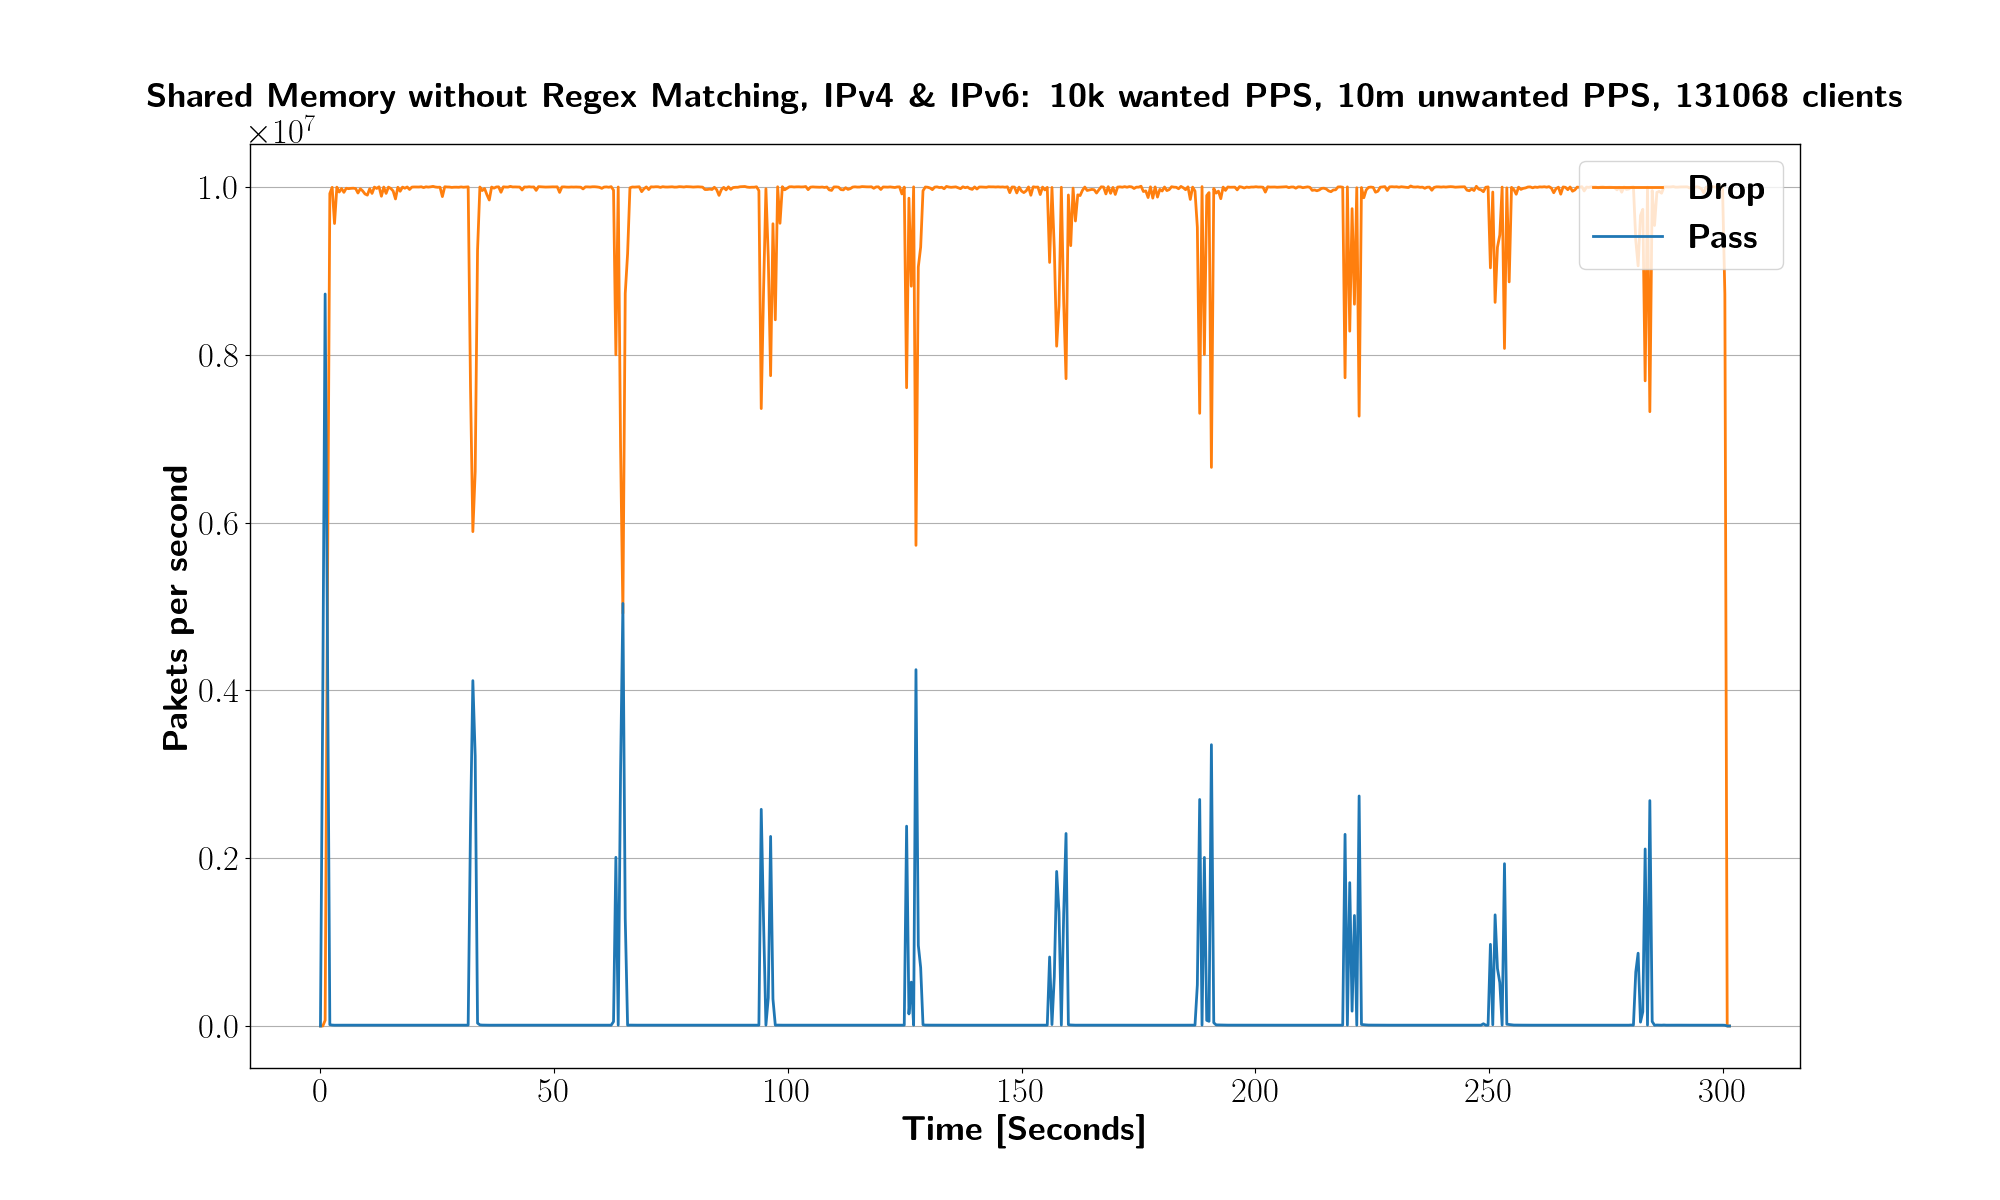
\includegraphics[width=1.2\textwidth]{images/simplefail2ban_shm_nr_ipv46_v10k_iv10m_c131068.png}}
	\end{tabular}
	\begin{tabular}{lllll}
		\toprule
		\textbf{Total packets [$10^6$]} & \textbf{Packets dropped [$10^6$]} & \textbf{Relative drop [\%]} & \textbf{Log messages [$10^6$]} & \textbf{CPU [seconds]} \\ \midrule 
		2989.56 & 2941.9 & 98.63 & 13.29 & 34.04 \\
		\bottomrule
	\end{tabular}
	\caption[Simplefail2ban, Shared Memory without Regex Matching]{Some text}
\end{figure}

